% AER-Article.tex for AEA last revised 22 June 2011
\documentclass[12pt]{article}

%%%%%% NOTE FROM OVERLEAF: The mathtime package is no longer publicly available nor distributed. We recommend using a different font package e.g. mathptmx if you'd like to use a Times font.
% \usepackage{mathptmx}
\usepackage{markdown}
\usepackage{adjustbox}
\usepackage{graphicx}
\usepackage{booktabs}
\usepackage{natbib}
\usepackage{multirow}
\usepackage{fontenc}
\usepackage{float}
\usepackage{threeparttable}
\usepackage{subcaption} % for subfigure/subtable style subcaptions
 \usepackage{hyperref}
\usepackage{pdflscape}
\usepackage{adjustbox}
\usepackage{rotating}
%\usepackage{fancyhdr}
\usepackage[margin=1in]{geometry}
%\pagestyle{fancy}
%\fancyhf{} % Clear header and footer
%\fancyfoot[C]{\textit{\small\thepage}} % Centered page number at the bottom
%\renewcommand{\headrulewidth}{0pt} % Centered page number at the bottom
%\pagestyle{fancy}
% Your document content here
\captionsetup[figure]{position=top}
\captionsetup[subfigure]{skip=6pt,justification=centering}
\raggedbottom

\usepackage{setspace}
\doublespacing
% The mathtime package uses a Times font instead of Computer Modern.
% Uncomment the line below if you wish to use the mathtime package:
%\usepackage[cmbold]{mathtime}
% Note that miktex, by default, configures the mathtime package to use commercial fonts
% which you may not have. If you would like to use mathtime but you are seeing error
% messages about missing fonts (mtex.pfb, mtsy.pfb, or rmtmi.pfb) then please see
% the technical support document at http://www.aeaweb.org/templates/technical_support.pdf
% for instructions on fixing this problem.

% Note: you may use either harvard or natbib (but not both) to provide a wider
% variety of citation commands than latex supports natively. See below.

% Uncomment the next line to use the natbib package with bibtex 
%\usepackage{natbib}

% Uncomment the next line to use the harvard package with bibtex
%\usepackage[abbr]{harvard}

% This command determines the leading (vertical space between lines) in draft mode
% with 1.5 corresponding to "double" spacing.

% Fix table caption style
\makeatletter
\renewcommand{\tablename}{Table}
\renewcommand{\thetable}{\@arabic\c@table}
\renewcommand{\fnum@table}[1]{\tablename~\thetable: }
\makeatother

% Fix figure caption style
\makeatletter
\renewcommand{\figurename}{Figure}
\renewcommand{\thefigure}{\@arabic\c@figure}
\renewcommand{\fnum@figure}[1]{\figurename~\thefigure: }
\makeatother


\title{WOW Factor: Measuring Labor Loss from a Negative Tourism Supply Shock in Iceland}
\date{}

\begin{document}

\maketitle
\clearpage

\begin{abstract}
Tourism-dependent economies face substantial risks when international visitor flows are disrupted, yet evidence on the short-run labor market effects of sudden tourism supply shocks remains limited. This paper exploits the sudden bankruptcy of WOW Air as a natural experiment that sharply curtailed international tourism to Iceland. Using a Bayesian Structural Time Series model, I estimate labor market outcomes relative to a counterfactual in which the airline did not exit. Nine months later, I find that the bankruptcy reduced international travel by more than 20\% and tourism employment (excluding air transport) by 8\%. At the national level, unemployment was nearly 50\% higher than would otherwise have been expected. These results highlight the vulnerability of tourism-dependent economies to sudden transport disruptions.
\\ 
\\
Keywords: tourism employment; air transport; tourism shocks; labor markets; island economies; causal inference
\end{abstract}
\clearpage

\section{Introduction}\label{sec:Introduction}
Tourism-dependent economies generate substantial employment and public revenue through visitor spending, but they also rely heavily on sustained international connectivity, creating exposure to external disruptions that can quickly destabilize local economies. When visitor flows contract, the effects are reflected in wages, tax revenues, and broader labor markets. These risks are especially acute in island destinations, where tourism often depends on a small number of transport links and limited alternative industries.

I study the abrupt bankruptcy of Icelandic airline WOW Air as a sharp and plausibly exogenous tourism supply shock. For an island economy with limited substitutes for international access, the collapse of a major low-cost airline provides a rare opportunity to isolate how reduced connectivity affects employment and broader economic activity. Using a Bayesian Structural Time Series (BSTS) model~\citep{brodersen_2015_inferring}, I estimate counterfactual outcomes in the absence of the shock.

This paper demonstrates two sides of the relationship between airlines and destination economies: the economic gains created by expanded connectivity and the labor market consequences when that connectivity is abruptly reduced. It shows not only the scale of disruption caused by such a shock, but also which sectors and workers are most exposed. For policymakers, understanding both the magnitude of these losses and who is most likely to bear them is essential for designing resilience strategies, preventing hard bankruptcies where possible, and distributing support effectively when disruption cannot be avoided.

I find that WOW Air’s collapse reduced passenger departures by more than 20\%, tourism employment by over 8\%, and national unemployment by nearly 50\% relative to the counterfactual path. These results provide causal evidence of how sudden airline exits affect labor markets in tourism-dependent economies and highlight the importance of resilience planning, carrier diversification, and labor market adjustment policies, while also demonstrating that even a low-cost carrier can serve as a critical pillar of local tourism economies.

\section{Literature Review}\label{sec:Literature}
The COVID-19 pandemic revealed the acute vulnerabilities of tourism-dependent economies, with international shutdowns exposing the fragility of over-reliance on a single sector. \citet{duro_2021_covid19} shows that regions with higher tourism concentrations experienced disproportionate exposure to pandemic losses. However, it also presented a seemingly ideal opportunity for researchers to observe responses to how regions and individuals respond to the unusual absence of tourism.  \citet{jczmyk_2023_impact} identify how tourist behaviors and choices shifted in response to health risks and uncertainty. \citet{yeh_2020_tourism} and \citet{kreiner_2020_national} evaluate optimal recovery strategies, while \citet{fotiadis_2021_the} and \citet{kare_2020_impact} provide forecasts of tourism impacts and recovery trajectories under varying conditions. Meanwhile, \citet{sigala_2020_tourism} reflects more broadly on the changed research landscape, emphasizing the unprecedented scope of the pandemic and the challenge of generalizing from its impacts. Taken together, this literature highlights how tourism reliance can create vulnerabilities for associated labor markets, but also how unique the pandemic was in both scale and global reach. At the same time, it leaves unresolved the question of replicability: while COVID-19 exposed the sector’s vulnerabilities in an extraordinary way, the shock was shaped by many confounding factors beyond tourism itself, making it difficult to entirely isolate effects or anticipate the size of future disruptions.

Beyond the pandemic, structural reliance on foreign tourism may create inherent economic vulnerabilities due to dependence on external visitor flows. \citet{nguyen_2021_the} find that a greater concentration of international tourism increases economic vulnerability, while \citet{canh_2020_domestic} show that domestic tourism can reduce it. \citet{wang_2022_international} identify a threshold effect: at lower income levels international tourism heightens vulnerability, while at higher incomes it promotes diversification. However, these studies rely on international panel regressions where vulnerability is measured through the Economic Vulnerability Index (EVI) \citep{feindouno_2016_the}, rather than observed economic responses. Because the EVI includes export concentration as a component, and international tourism is classified as an export, this presents a mechanical calculation. Moreover, the index captures exposure to shocks but not resilience to withstand them. At the same time, a complementary literature highlights the resilience of tourism demand following crises that temporarily dissuade travel. \citet{saleh_2011_do} document that tourism shocks in Thailand are transitory, and \citet{yucel_2020_are} extend this finding to the top 20 tourism-receiving countries, with demand reverting once structural breaks are accounted for. \citet{morakabati_2019_a} shows that, following the Arab Spring, regional international tourism receipts recovered faster than the broader economy. These studies illustrate both the fragility and resilience of the sector, but provide little causal evidence of how sudden supply disruptions affect labor markets or how policy may mitigate their impacts.

Tourism has also been closely linked to economic growth and labor market performance. \citet{gwenhure_2017_tourism} synthesize this literature into four competing hypotheses regarding the relationship between tourism and growth, with somewhat stronger support for the theory that tourism-led growth is a verifiable source of income growth. Within island contexts, \citet{seetanah_2011_assessing} find that tourism contributes more significantly to economic growth than in other developing and developed economies. While this literature highlights tourism as a viable strategy for growth and development, it often gives less attention to the vulnerabilities created by heavy reliance on external visitor flows and how labor markets adjust when those flows suddenly contract.

For island economies, international tourism flows are often sustained by a small number of airlines and routes, making air connectivity central to both growth and vulnerability. Many of these routes are served by low-cost carriers (LCCs) operating on thin margins. \citet{alves_2017_price} describe how LCCs function as price-discriminating complements, targeting more price-sensitive travelers and expanding total visitor flows rather than simply reallocating existing demand. Case studies across Saudi Arabia, Poland, Spain, New Zealand, and Italy show that LCC entry creates new, previously uncontested markets \citep{alsumairi_2017_a, pulina_2010_have, rey_2011_effect, hongtsui_2017_does, verarebollo_2009_spread}. This expansion can deepen dependence on visitor flows that may disappear if those routes are withdrawn. Because other carriers are often unable to replicate the same capacity or market reach, LCC exits can create sharp supply-side contractions and provide a clean setting for identifying how tourism shocks propagate through labor markets.

Understanding the impacts of sudden losses in tourism flows has become increasingly important, particularly following the COVID-19 pandemic, which demonstrated how quickly declines in visitor arrivals can generate labor market and fiscal pressures. Governments and destination managers need to know not only whether these disruptions matter, but how large the effects are and which sectors and workers are most exposed in order to better plan for resilience and recovery. While the literature strongly establishes tourism as an important driver of growth and employment, and increasingly acknowledges the vulnerabilities created by heavy reliance on external visitor flows, there is less clean causal evidence showing how these shocks affect local economies in an exogenous setting. This paper addresses that gap by examining the unexpected bankruptcy of WOW Air in Iceland. Its abrupt collapse created a sharp reduction in international access that was not easily substituted, providing a rare opportunity to isolate how the loss of tourism flows affects employment, wages, and broader economic activity.

\section{Data}\label{sec:data}
\subsection{Choice of Controls} 
Greenland, Denmark, Norway, and the Faroe Islands are used as control groups to estimate Iceland’s counterfactual. These countries were selected based on geographic proximity and similarities in size, tourism concentration, seasonality, and export reliance, as summarized in Table \ref{tab:summary_table}. Sweden, Ireland, and the United Kingdom were also considered, but ultimately excluded due to larger differences in size, economic diversification, and geography. While Greenland and the Faroe Islands are autonomous territories within the Kingdom of Denmark, Denmark itself is included as a separate control due to its role as a primary regional trading partner whose economic fluctuations often co-vary with those of Iceland and its territories. As shown in Appendix \ref{sec:Robustness}, the estimated impacts are robust to alternative specifications of the control group.

\begin{table}[htbp]
\centering
\caption{Forecasted Change in Tourism From Different Coefficient Groups}
\resizebox{\textwidth}{!}{%
\begin{tabular}{lcccccccc}
    \toprule
          & \textbf{Iceland} & \textbf{Faroe Islands} & \textbf{Greenland} & \textbf{Norway} & \textbf{Denmark} & \textbf{Sweden} & \textbf{Ireland} & \textbf{UK} \\
    \midrule
    Nordic Country & X & X & X & X & X & X & - & - \\
    Distance to Iceland (mi.) & - & 181 & 272 & 339 & 917 & 774 & 670 & 492 \\
    Seasonality (Difference Between Longest \& Shortest Day) & 17:02 & 14:37 & 17:04 & 12:56 & 10:31 & 12:32 & 9:30 & 8:48 \\
    Population 2018 (million) & 0.35 & 0.05 & 0.06 & 5.31 & 5.79 & 10.18 & 4.87 & 66.46 \\
    Annual Tourists per Capita (2013) & 2.78 & 2.41 & 1.22 & 0.94 & 4.72 & 1.14 & 1.79 & 0.52 \\
    Annual Tourists per Capita (2018) & 7.05 & 3.66 & 1.52 & 1.07 & 5.32 & 0.73 & 2.24 & 0.61 \\
    5 Year Change in Tourism Per Capita & 154\% & 52\% & 25\% & 14\% & 13\% & -36\% & 26\% & 16\% \\
    Fish, Animals, and Animal Products as Export Product Share (2009) & 38\% & 87\% & 56\% & 6\% & 11\% & 2\% & 4\% & 1\% \\
    \bottomrule
    \end{tabular}%
}
<<<<<<< Updated upstream
\footnotesize\begin{tablenotes}[Source:]
=======
\tiny\begin{tablenotes}[Source:]
>>>>>>> Stashed changes
1. Globefeed.com, 2. US Naval Observatory Astronomical Applications Department, 3. Nordicstatistics.org, 4. World Bank
\end{tablenotes}
\end{table}


\subsection{Dataset}

I assemble a monthly cross-national time-series dataset of tourism and economic indicators from national statistical agencies.\footnote{Iceland: \textit{hagstofa.is} (2024); Faroe Islands: \textit{hagstova.fo} (2024); Greenland: \textit{bank.stat.gl} (2024); Denmark: \textit{statbank.dk} (2024); Norway: \textit{ssb.no} (2024).} Nordic regional data was collected from \textit{nordicstatistics.org}.\footnote{\textit{nordicstatistics.org} (2024).} Where official monthly data were unavailable, I supplemented with the World Bank Open Data Portal\footnote{\textit{data.worldbank.org} (2024).} and The Global Economy.\footnote{\textit{theglobaleconomy.com} (2024).} Indicators were excluded if coverage was incomplete across the pre- or post-intervention period, if they were linear combinations of other variables, or if they were subject to high measurement noise (e.g., survey data with small samples).  


\subsection{Data Availability}\label{sec:Data Availability}

Limitations in uniform cross-country data availability shaped the empirical approach. The synthetic control method of \citet{abadie_2003_the} requires identical outcome variables across treatment and control groups, a condition not met here. Our dataset's reported indicators vary in scope, frequency, and level of disaggregation across countries. For example, Greenland and the Faroe Islands provide relatively few monthly indicators, and those that are available are often defined differently from Iceland’s series. In some cases, measures are reported only in aggregate form, while in others they are disaggregated by sector, age, or region, reducing comparability across countries. For instance, Iceland reports both total and sector-specific employment and wage measures, including total employees, employees in tourism, and employees in accommodation and food services, whereas Greenland provides only an aggregate employment figure without any breakdown by sector or industry. Even so, indicators from control countries may still serve as informative predictors of related outcomes in Iceland (e.g., passenger arrivals in Greenland may co-vary with hotel check-ins in Iceland). These information asymmetries are summarized in Table \ref{tab:information_asymmetry}.

 As discussed further in Section \ref{sec:methods}, I group available variables into topic areas and use them as covariate groups in the model’s calibration. Because the Bayesian Structural Time Series (BSTS) framework is able to self-select predictive covariates, results remain consistent whether I include the full set or only the most relevant indicators. For example, I use the Tourism \& Transportation Topic area from Table \ref{tab:information_asymmetry} to predict tourism outcomes. But if I also include additional information about local fuel use and national accounting, only the most relevant covariates are ultimately selected (depicted in Table \ref{tab:choice_control_coeffs}). 

\clearpage
\begin{tabular}{lrrrrrr}
\toprule
Passenger Series & Relative Impact (\%) & 9-Month Cumulative Impact & 95\% CI Upper & 95\% CI Lower & p-value & RMSE (pre-period) \\
\midrule
Total Passengers & -20.63*** & -533,643 & -251,386 & -942,546 & 0.0002 & 13,530 \\
\midrule
Icelandic Passengers & -16.70*** & -100,771 & -23,111 & -180,957 & 0.0010 & 2,905 \\
Foreign Passengers & -22.75*** & -461,168 & -211,729 & -831,090 & 0.0002 & 11,895 \\
\midrule
United States & -42.29*** & -272,408 & -141,886 & -383,908 & 0.0002 & 6,063 \\
Canada & -36.59*** & -32,481 & -20,250 & -44,873 & 0.0002 & 1,153 \\
Sweden & -27.51*** & -12,861 & -6,352 & -19,808 & 0.0008 & 499 \\
Italy & -27.34** & -13,537 & 1,601 & -24,885 & 0.0410 & 442 \\
Spain & -26.75** & -17,775 & -1,284 & -31,582 & 0.0153 & 627 \\
Poland & -25.14*** & -25,728 & -15,218 & -35,515 & 0.0002 & 568 \\
United Kingdom & -18.29* & -33,566 & 10,633 & -80,275 & 0.0696 & 3,290 \\
Germany & -18.21** & -24,022 & 1,594 & -49,395 & 0.0364 & 1,427 \\
Switzerland & -18.09** & -4,816 & 448 & -10,903 & 0.0384 & 287 \\
Russia & 16.31* & 2,115 & 5,027 & -901 & 0.0778 & 171 \\
Norway & -15.16** & -5,735 & -344 & -11,590 & 0.0200 & 306 \\
Finland & -14.88** & -3,100 & 116 & -6,500 & 0.0297 & 260 \\
France & -12.17 & -10,769 & 5,094 & -29,234 & 0.1000 & 851 \\
Netherlands & -10.70** & -4,186 & 617 & -9,561 & 0.0475 & 419 \\
Denmark & -10.33** & -4,614 & 610 & -9,752 & 0.0408 & 340 \\
Japan & 6.51 & 765 & 4,346 & -2,797 & 0.3503 & 268 \\
China & -5.45 & -4,453 & 10,830 & -24,292 & 0.3040 & 1,027 \\
\bottomrule
\end{tabular}

\clearpage

A further issue is recency bias in data availability. As shown in Figure \ref{fig:recent_information_bias}, by 2014 roughly 80\% of covariates are observed at monthly frequency, allowing richer model calibration. This creates a trade-off where if we  start the pre-intervention training period later, it reduces the observed time-series trend but increases the number of usable covariates. This dynamic is illustrated in Figure \ref{fig:time_calibration}.  

\begin{figure}[htbp]
\centering
\caption{Recent Information Bias}\label{fig:recent_information_bias}
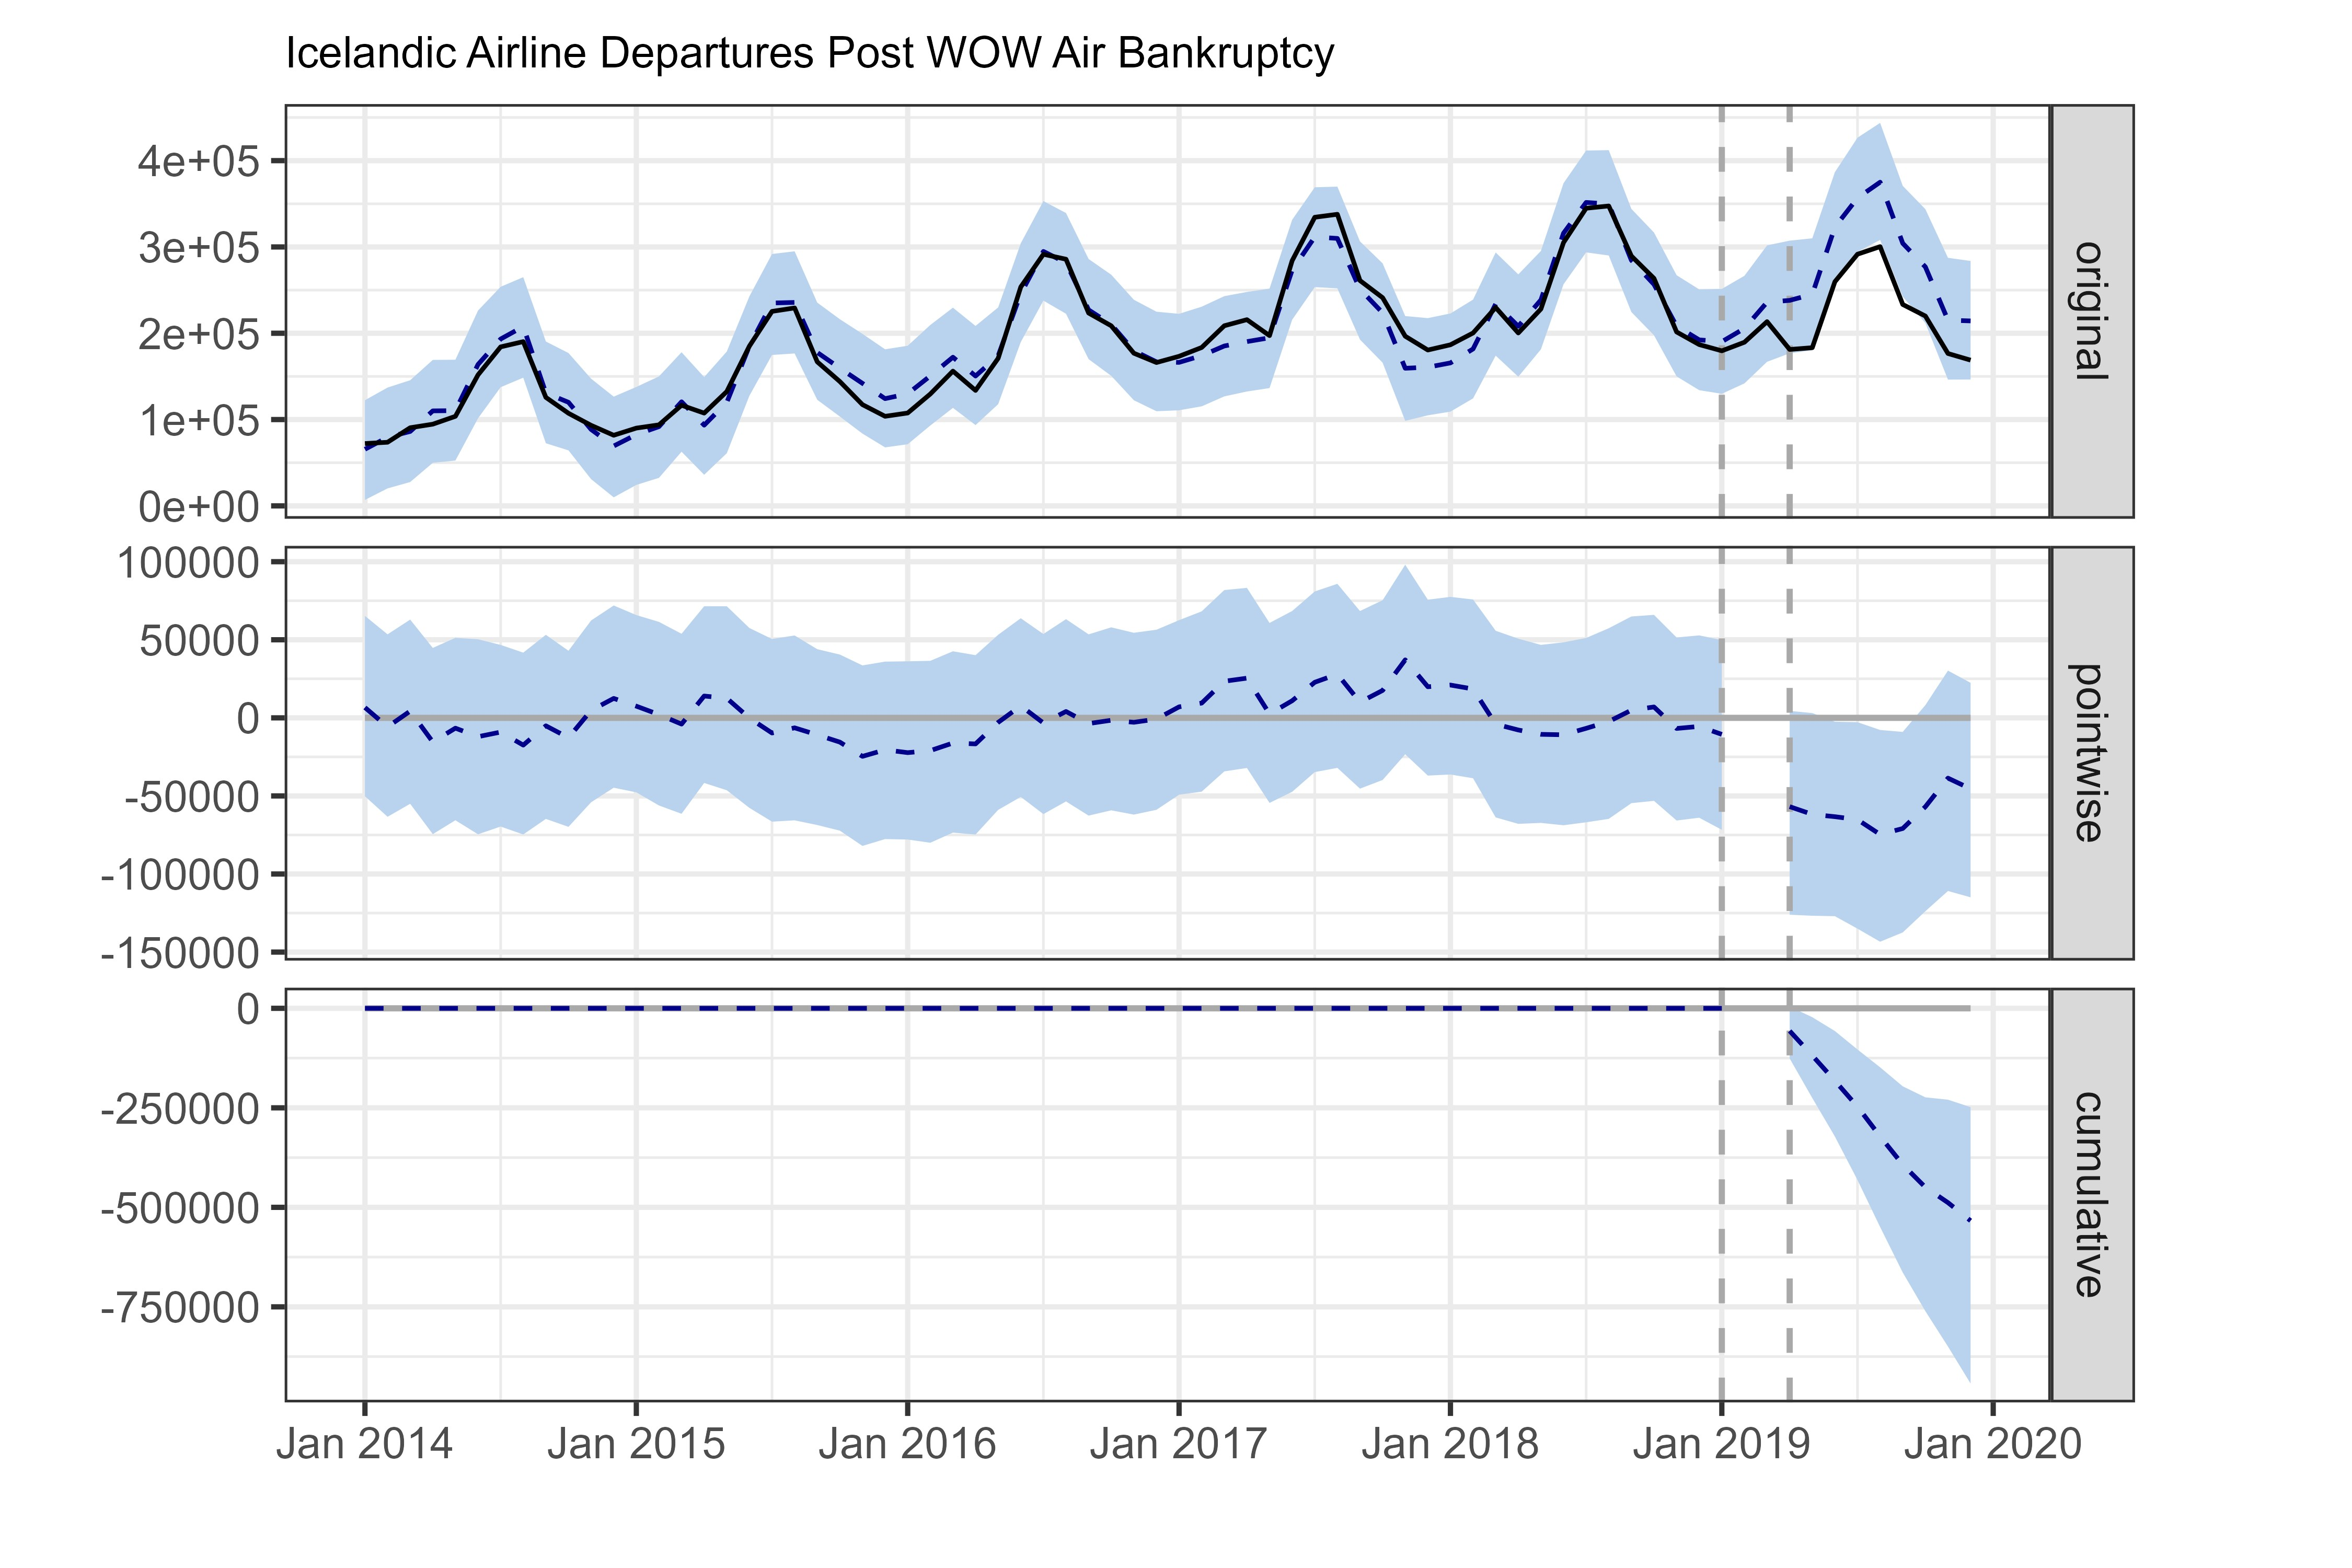
\includegraphics[width=0.7\textwidth,height=0.4\textheight]{Figures/Figure 1.jpg}
\parbox{\linewidth}{\footnotesize \centering\textit{Note:} Plot of the percent of covariate fields without missing values by date.}
\end{figure}




\section{Methodology}\label{sec:methods}
\subsection{Empirical Design}

The objective is to estimate the effect of the WOW Air bankruptcy on Iceland’s outcomes by comparing observed series to a counterfactual path that would have occurred in its absence. Formally, the causal effect at time $t$ is the difference between the observed outcome for Iceland ($Y_{I,t}$) and the unobserved counterfactual ($Y_{N,t}$), where the WOW Air bankruptcy did not happen. Since $Y_{N,t}$ is not observed, it must be estimated from a model informed by Iceland’s own pre-trends and by contemporaneous outcomes in unaffected countries.

I implement a Bayesian Structural Time Series (BSTS) model following \citet{brodersen_2015_inferring}. Let the pre-intervention training period be $t=1,\dots,n$, where $n$ is January 2019. The post-intervention forecasting period begins with $t=n+3,\dots,m$, where the two-month buffer $(n+1,n+2)$ accounts for WOW Air’s gradual route reductions before its final bankruptcy mid-March 2019. The counterfactual outcome for Iceland is modeled as:
\begin{align}
Y_t &= \mu_t + \tau_t + \sum_{j \in \mathcal{J}} x_{j,t}\beta_j + \varepsilon_t, \quad t = 1,\dots,m \label{eq:obs} \\
\mu_{t+1} &= \mu_t + \delta_t + \eta_{\mu,t}, \quad t = 1,\dots,n \label{eq:level} \\
\delta_{t+1} &= \delta_t + \eta_{\delta,t}, \quad t = 1,\dots,n \label{eq:slope} \\
\tau_{t+1} &= -\sum_{k=1}^{S-1}\tau_{t-k} + \eta_{\tau,t}, \quad S=12 \label{eq:season}
\end{align}

Equation \eqref{eq:obs} is the observation equation. The observed outcome (e.g., international passenger departures, tourism employment) is expressed as the sum of latent components plus noise, with contemporaneous controls $x_{j,t}$ from unaffected countries $j \in \mathcal{J}$. Equation \eqref{eq:level} defines a local level $\mu_t$, representing Iceland’s underlying trend. Equation \eqref{eq:slope} introduces a local slope $\delta_t$, which allows the trend to change over time. Equation \eqref{eq:season} adds a seasonal component $\tau_t$ with $S=12$ months, capturing Iceland’s highly seasonal tourism cycle. Gaussian disturbances $\varepsilon_t, \eta_{\mu,t}, \eta_{\delta,t}, \eta_{\tau,t}$ are mutually independent.

Control selection is handled via spike-and-slab priors, which induce sparsity and allow the model to include only those covariates that improve predictive fit in the pre-treatment period. Intuitively, the “spike” shrinks irrelevant coefficients toward zero while the “slab” allows nonzero values for genuinely predictive controls, letting the model probabilistically switch covariates on or off during estimation. This prevents overfitting while highlighting the controls that truly drive Iceland’s pre-2019 tourism trajectory. Figure~\ref{fig:coefficients_arrivals_plot} summarizes the posterior inclusion probabilities (PIPs) from the primary model, indicating which covariates were most consistently selected across posterior draws and their coefficient magnitudes.

\begin{figure}[hbtp]
    \centering
    \caption{Posterior Inclusion Probabilities}
    \label{fig:coefficients_arrivals_plot}

    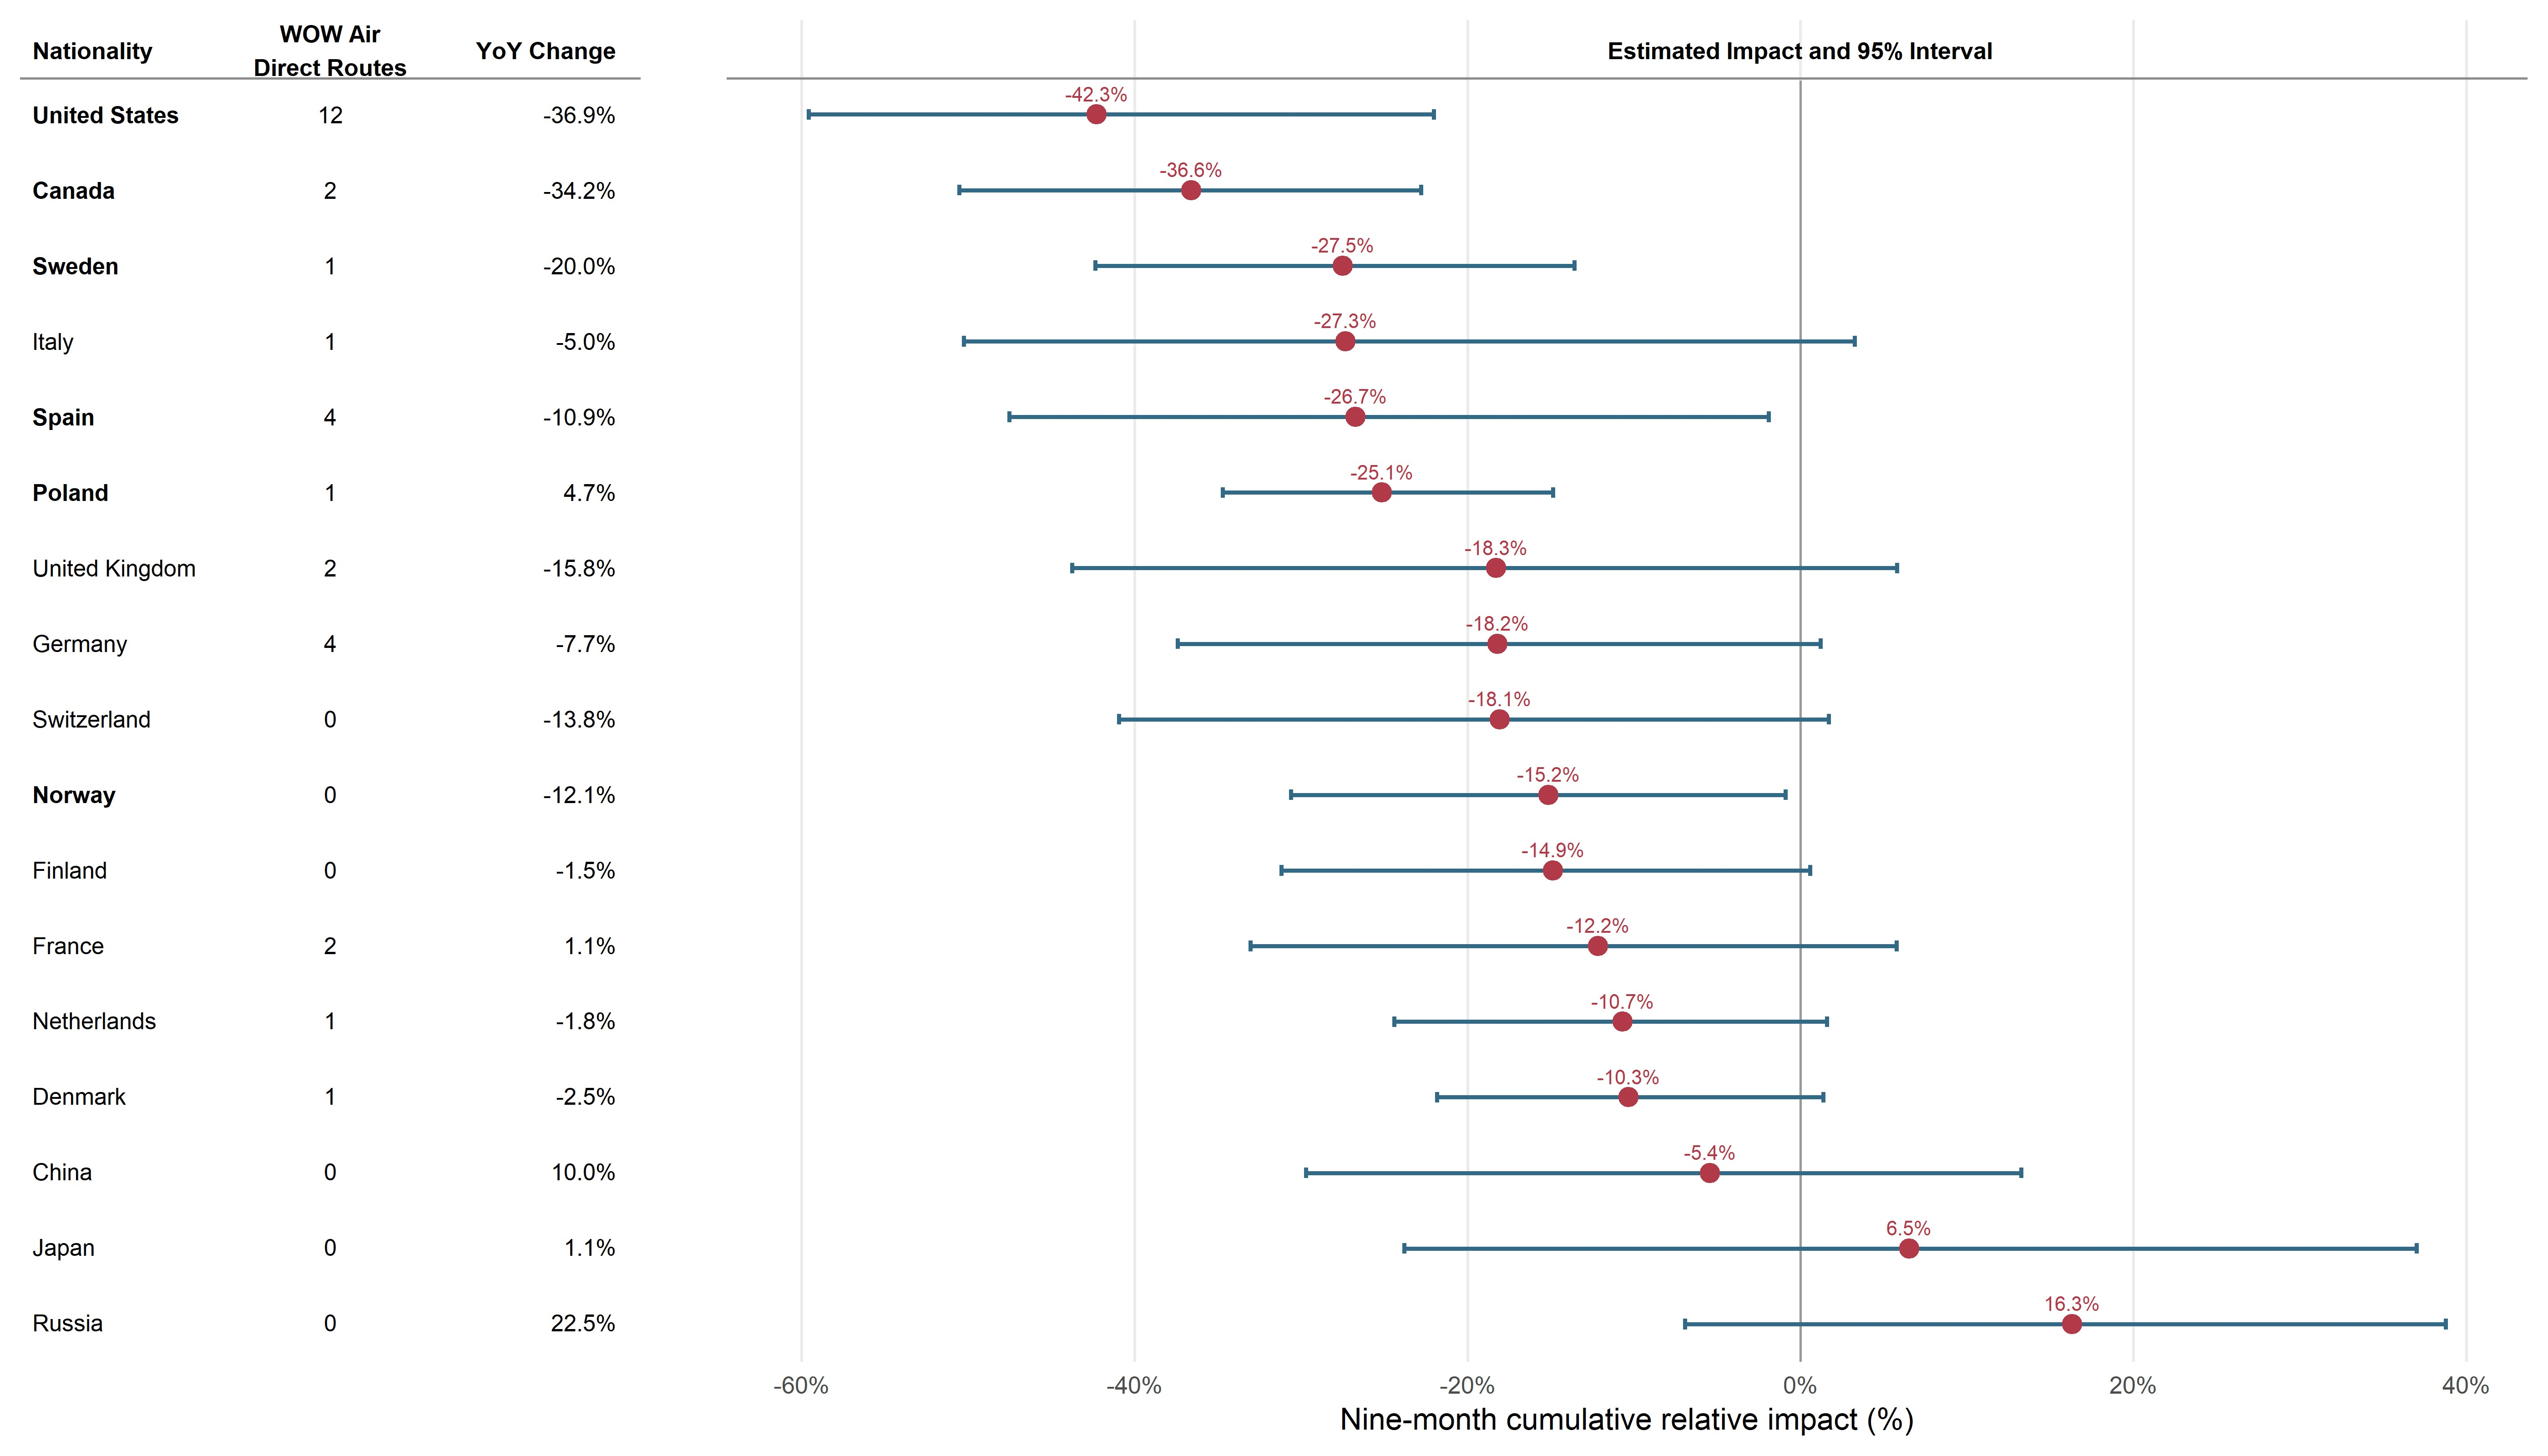
\includegraphics[width=1\textwidth]{Figures/Figure 2.jpg}

    \vspace{0.3em}

    {\centering
    \parbox{0.9\textwidth}{\tiny
    \setstretch{1}
    \textit{Note:} Each cell represents a separate regression. The country listed under Treated Country is who we are applying the treatment to. All others (less Iceland) are used as controls groups. The columns represent varying length of training periods used. 1 year prior compares the treatment effect using 1 year of pre-trend data. The number of stars denotes the significance level of the coefficient estimates based on p-values, where *** indicates $p<0.01$, ** indicates $p<0.05$, and * indicates $p<0.10$.}\par}
\end{figure}


\paragraph{Model Calibration}
To implement the model, I use the \texttt{CausalImpact} package in R \citep{brodersen_2015_inferring}. Being a flexible tool, it allows for numerous user calibrating inputs. The choice of pre-intervention window reflects a trade-off between having longer training periods and ensuring rich covariate coverage. Data availability improves substantially after 2014 (see Figure \ref{fig:recent_information_bias}), so I test specifications beginning in each year from 2000–2018, with treatment fixed in April 2019. Figure \ref{fig:time_calibration} reports cumulative impacts across these specifications. The estimates vary somewhat by training start date but consistently indicate a large causal reduction in airline departures. Given structural changes in Iceland’s economy toward tourism beginning around 2012,\footnote{WOW Air began operations in May 2012; see \citet{diebold_1987_structural} for discussion of structural breaks.} I adopt 2014 as the start year for the main analysis. This balances adequate time-series coverage with robustness and placebo validity. Across all training windows (2000–2018), the mean cumulative impact is approximately –487,000 passengers and the median –458,000, with the 2014 specification yielding an estimated –538,000 passengers.

\begin{figure}[h!]
    \centering
    \caption{Cumulative effects across pre-periods}
    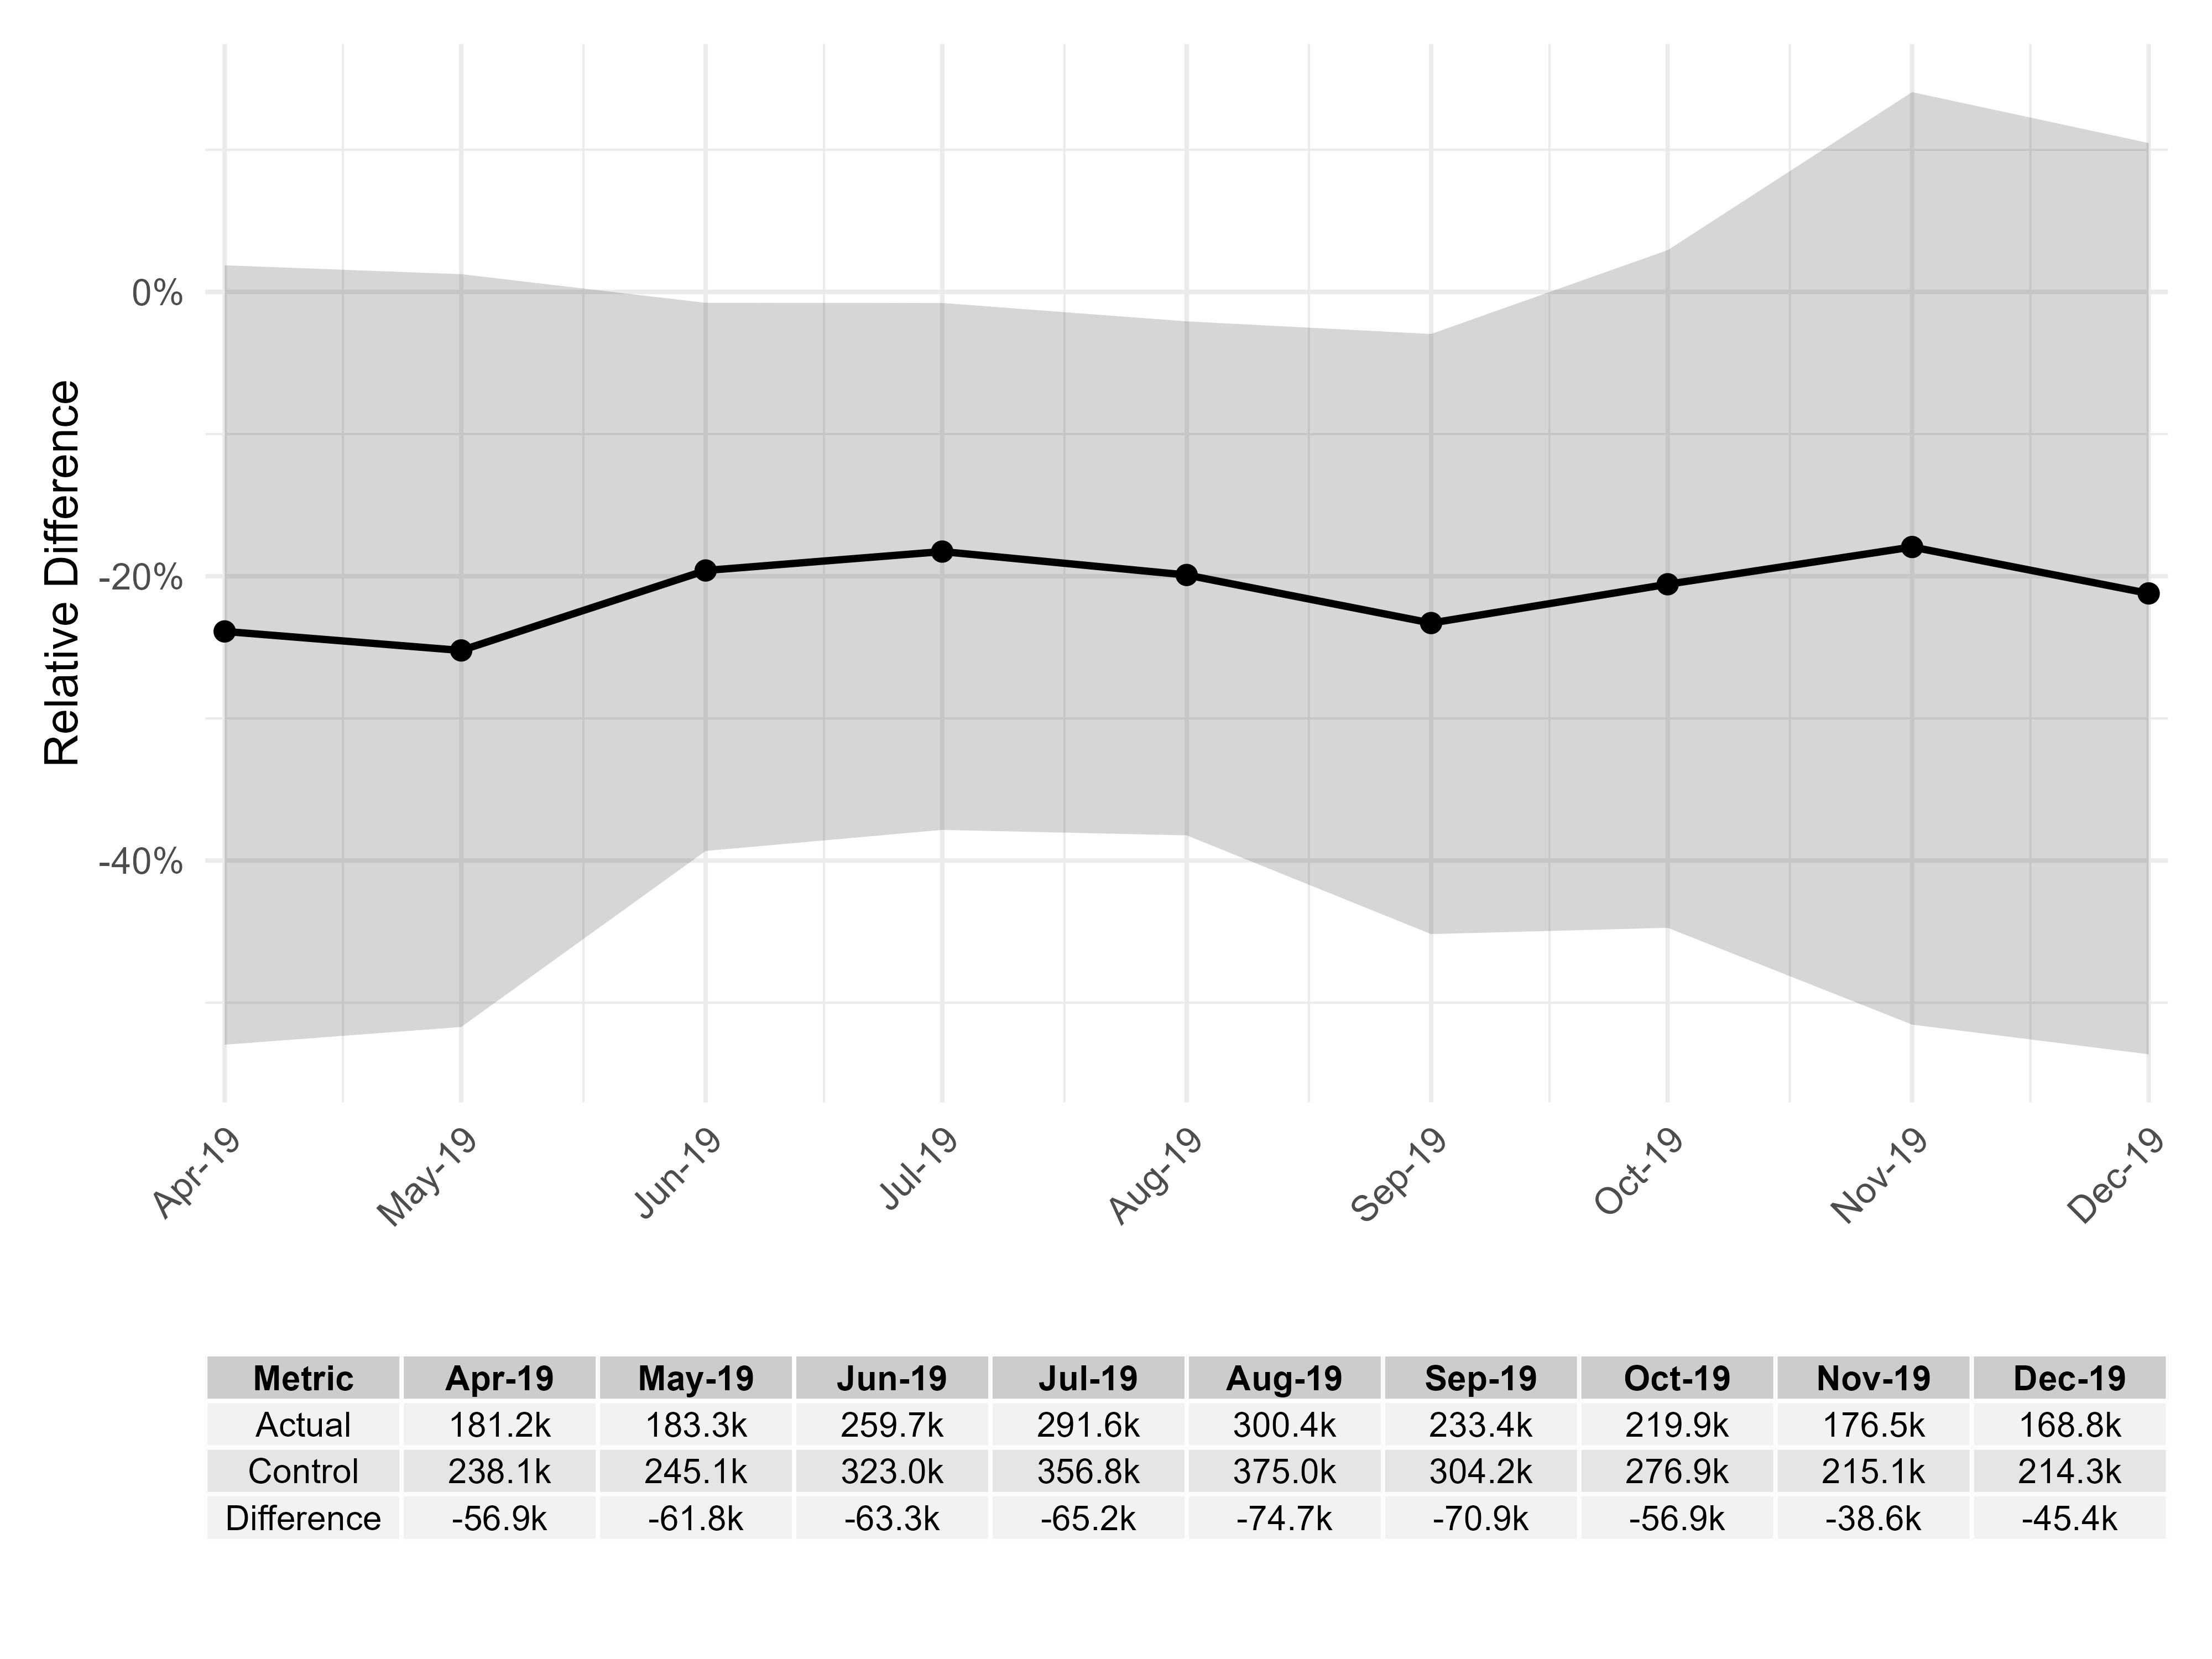
\includegraphics[width=\textwidth]{Figures/Figure 3.jpg}
    \label{fig:time_calibration}
    
    \begin{minipage}{\textwidth}
        \footnotesize \textit{Figure Statistics:}\\
        Median cumulative change: --458,000 departing passengers.\\
        Mean cumulative change: --487,000 departing passengers.\\
        2014 estimate: --538,000 departing passengers.
    \end{minipage}
\end{figure}

The forecasting window begins in April 2019 ($t=n+3$) and continues through December 2019 ($m$). Excluding February and March ($n+1,n+2$) is essential because these months represent a transitory phase when WOW Air first reduced routes and then ceased operations mid-March, making them unsuitable for isolating the causal shock. Covariates $x_{j,t}$ are drawn from Nordic and near-Nordic economies, selected from the topic areas summarized in Table \ref{tab:information_asymmetry}, ensuring economic relevance and avoiding implausible predictors. Seasonality is modeled explicitly with a monthly component ($S=12$), reflecting the strong peaks and troughs in Arctic tourism activity. All other hyperparameters follow the defaults recommended by \citet{brodersen_2015_inferring}.



\section{Results}\label{sec:results}
\subsection{Passenger Travel Impacts}

\begin{figure}[h]
\caption{Decline in Airline Passengers}
\centering
    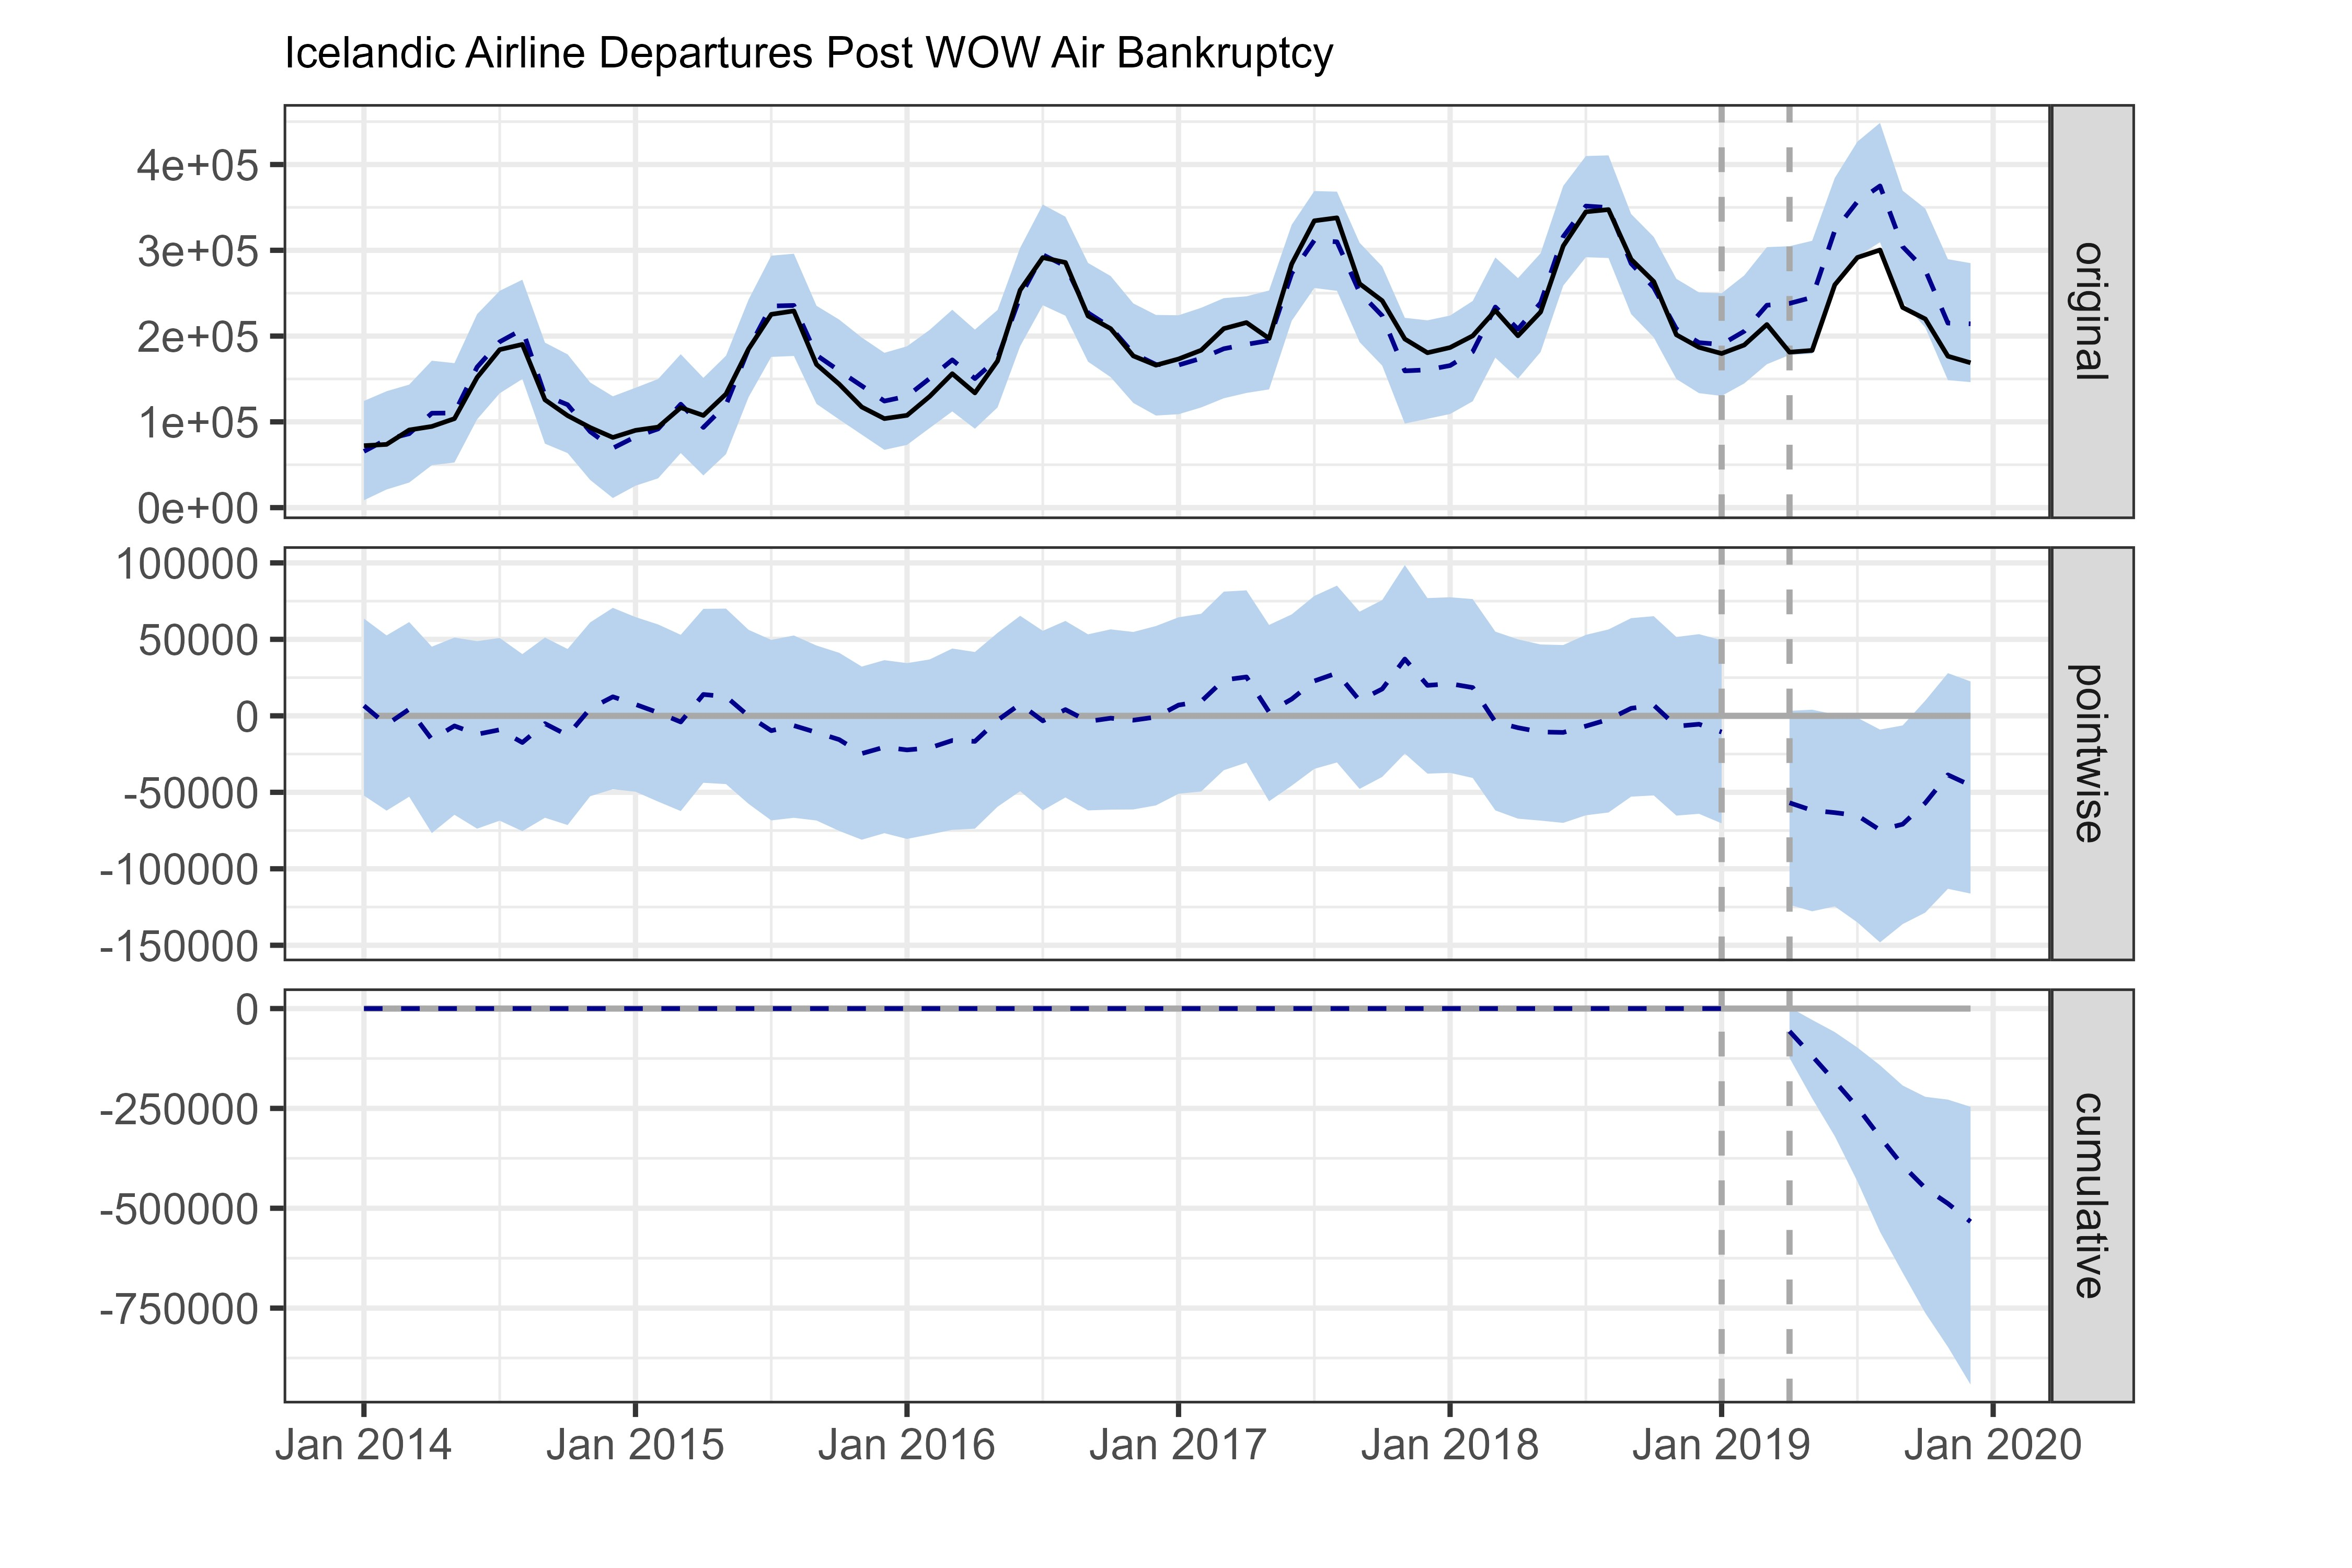
\includegraphics[width=0.8\textwidth]{Figures/Figure 4.jpg}\
\begin{minipage}{0.7\textwidth}
\footnotesize \textit{Note:} Departures are measured as the number of persons passing through international security. The solid line shows observed values, and the dashed line shows the synthetic counterfactual; shaded areas indicate uncertainty.
\end{minipage}
\label{fig:primary_arrivals_plot}
\end{figure}

This section begins by analyzing the impact of the WOW Air closure on passenger travel, which provides both the clearest channel through which the bankruptcy affected the economy and an important test of the empirical method. If the modeling approach cannot clearly recover the well-documented reduction in international passengers, confidence in the downstream labor results would be limited. Conversely, demonstrating that the model captures the contraction in passenger flows in situations where we expect it, but not in placebo situations,  validates the method and provides a necessary foundation for interpreting the labor outcomes.

Figure \ref{fig:primary_arrivals_plot} shows the estimated counterfactual number of passengers compared to observed departures as well as the monthly and cumulative differences. In the nine months following the bankruptcy, approximately 2.07 million passengers departed Iceland, compared to a counterfactual estimate of 2.60 million passengers in a synthetic Iceland where the bankruptcy did not occur. This implies about 534,000 fewer passengers than would have been expected, a reduction of roughly 20.6\%. Figure \ref{fig:fig_table_grouped} shows the same results broken down by passenger citizenship. Foreign visitors account for the majority of this decline: relative losses were 4\% larger for foreigners than for Icelandic residents, and in absolute terms the contraction in foreign passengers was nearly four times greater. These patterns align with the expectation that WOW Air’s exit would disproportionately affect international tourism flows with strong implications for lost export revenue. 


\begin{figure}[htbp]
\caption{Impacts on Passenger Counts by Nationality}
\label{fig:fig_table_grouped}
\centering
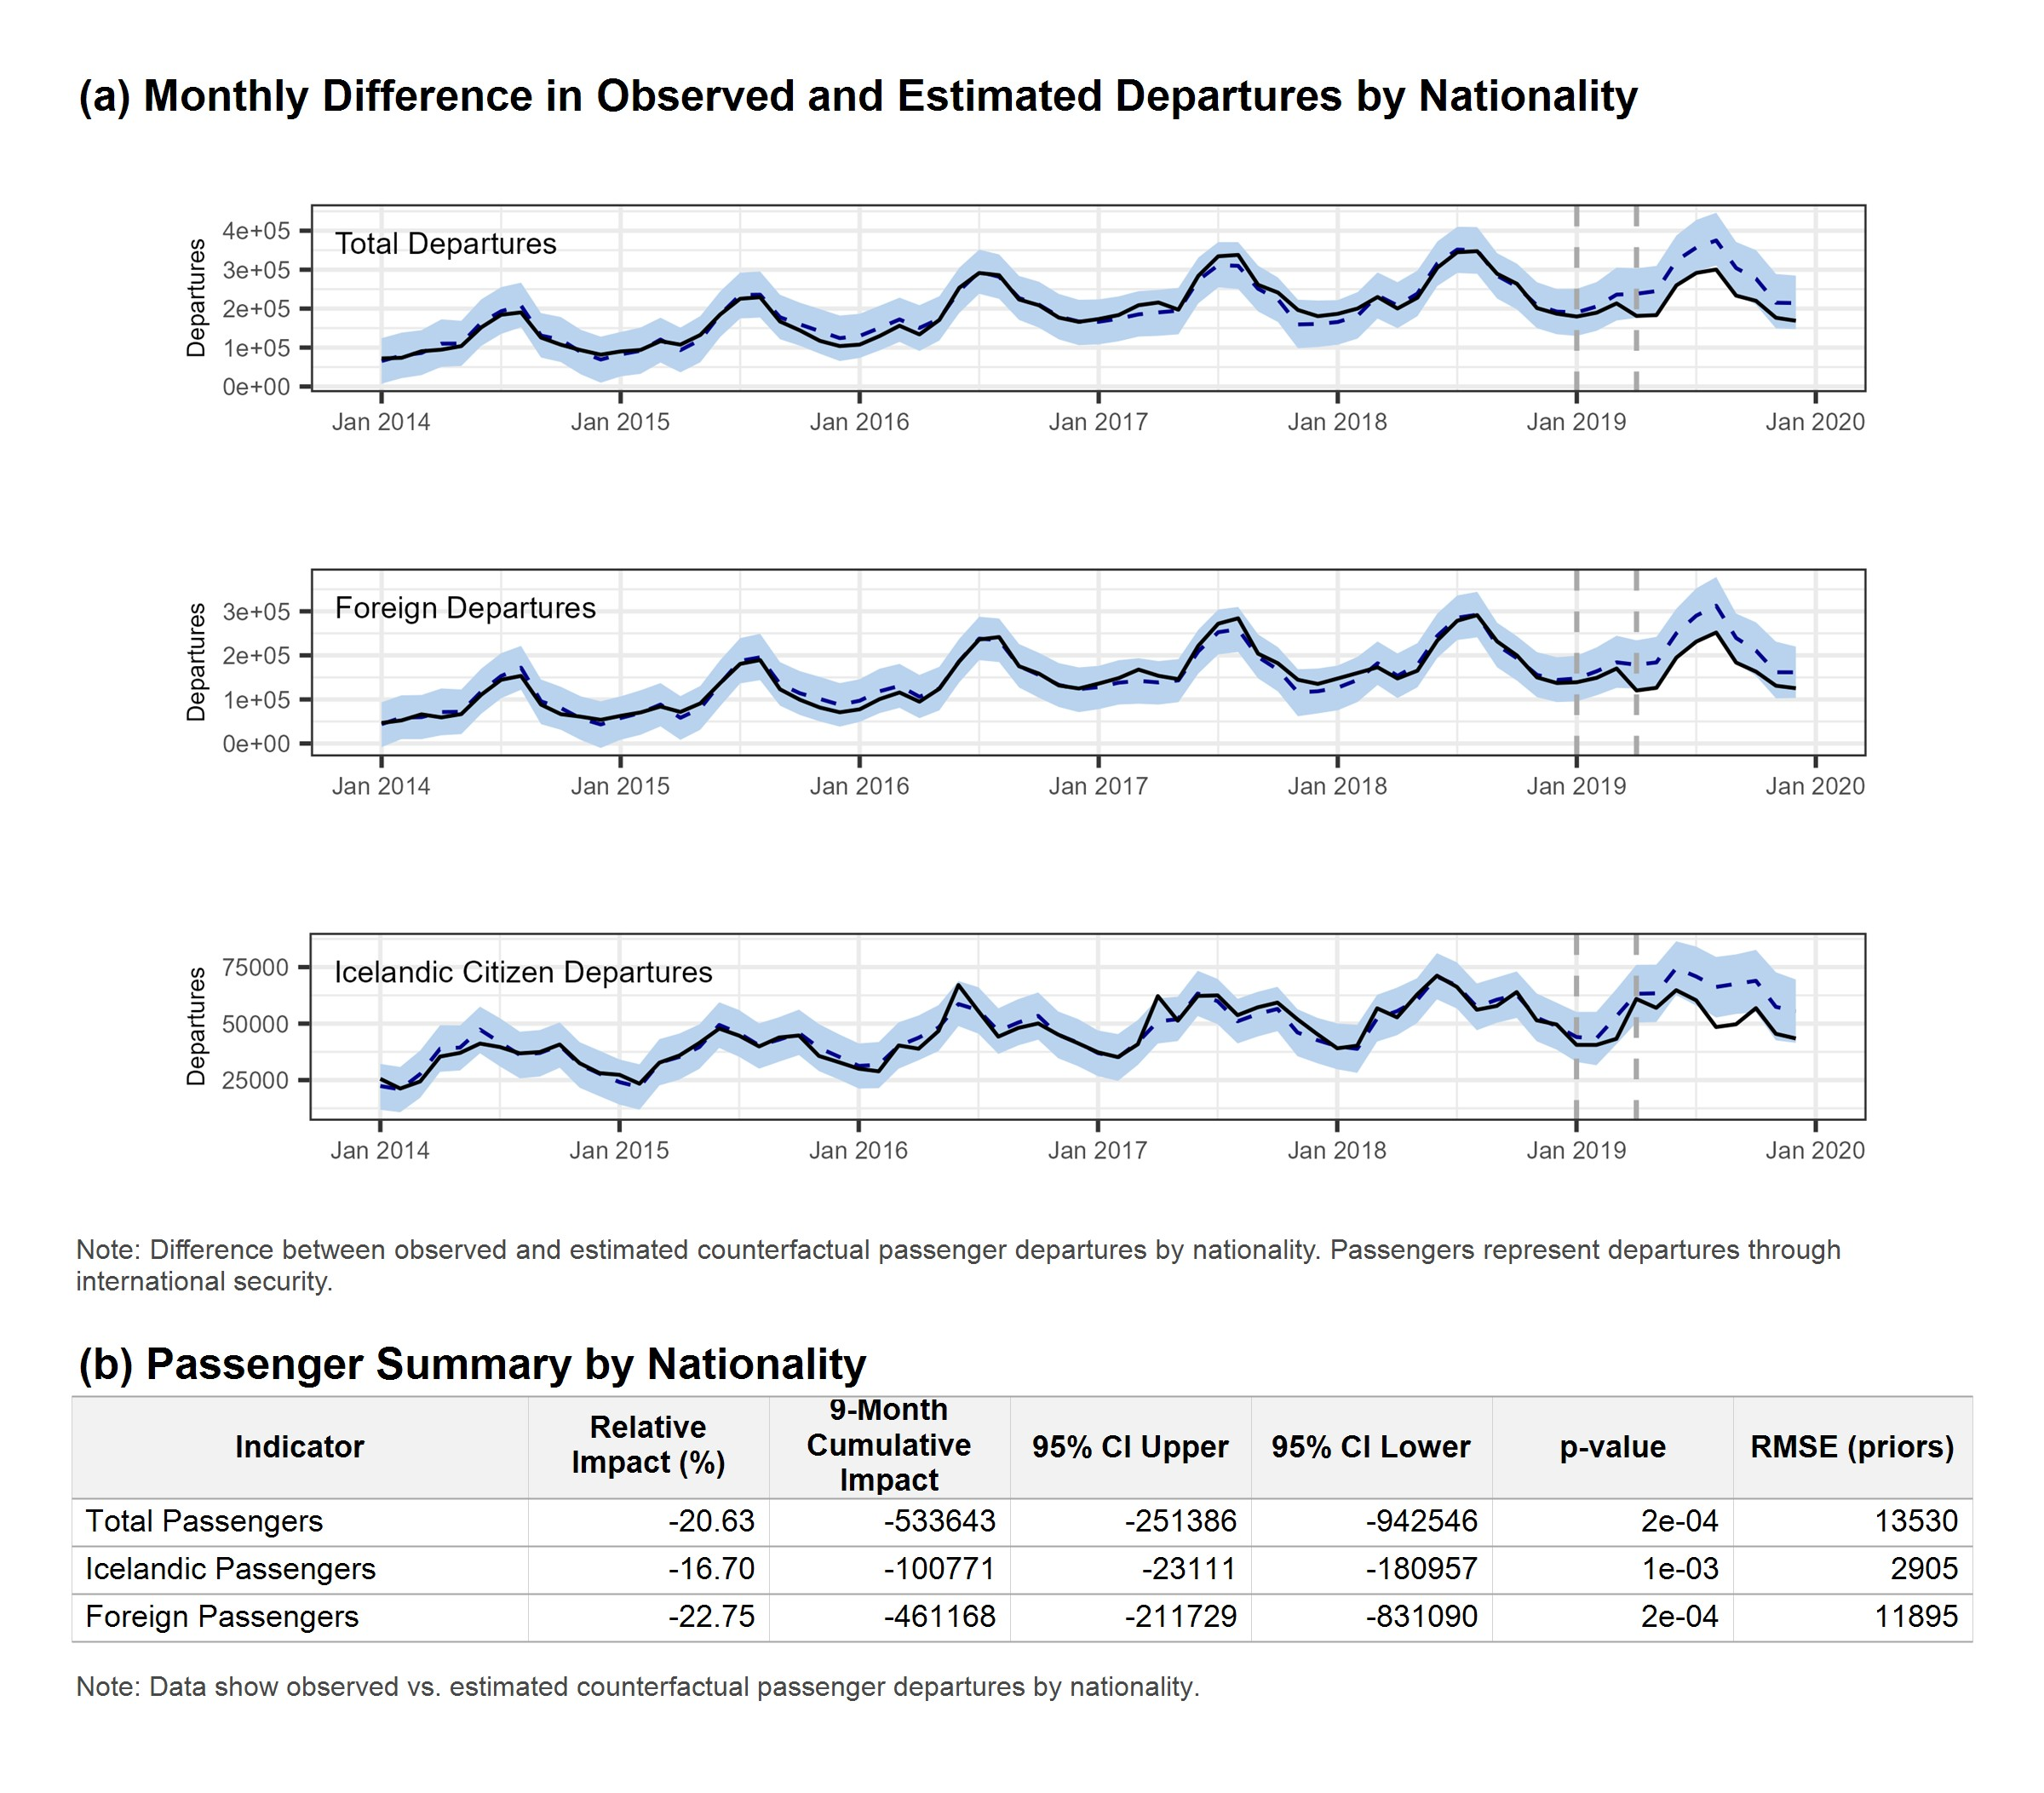
\includegraphics[width=\textwidth]{Figures/Figure 5.jpg}
\end{figure}

Figure \ref{fig:monthly_diff_plot} further illustrates these effects by expressing departures as a percentage deviation from the model’s counterfactual estimate. The solid line shows observed monthly differences, with the shaded region indicating the 95\% credible interval. Departures remained consistently below expected levels by roughly 15–25\% throughout 2019, with little sign of recovery even toward the end of the year. The table below the plot reports actual, predicted, and difference values for each month, reinforcing that the gap persisted across all months following the collapse.

While this pattern is not formally tested, the results suggest that the lost capacity was not easily substituted by other carriers during this period. This interpretation is consistent with the broader literature on low-cost carriers, which emphasizes that such airlines often stimulate their own demand and serve distinct market segments not readily filled by legacy carriers \citep{alsumairi_2017_a,pulina_2010_have,rey_2011_effect,hongtsui_2017_does,verarebollo_2009_spread,khan_2019_evolving}. Although exploratory, the persistence of the gap indicates that WOW Air played a distinctive role in sustaining international travel demand to and from Iceland, with meaningful implications for the country’s tourism-driven export sector.

\begin{figure}[h]
\caption{Monthly Arrivals Relative to Counterfactual (\% Higher or Lower Than Expected)}
\centering
    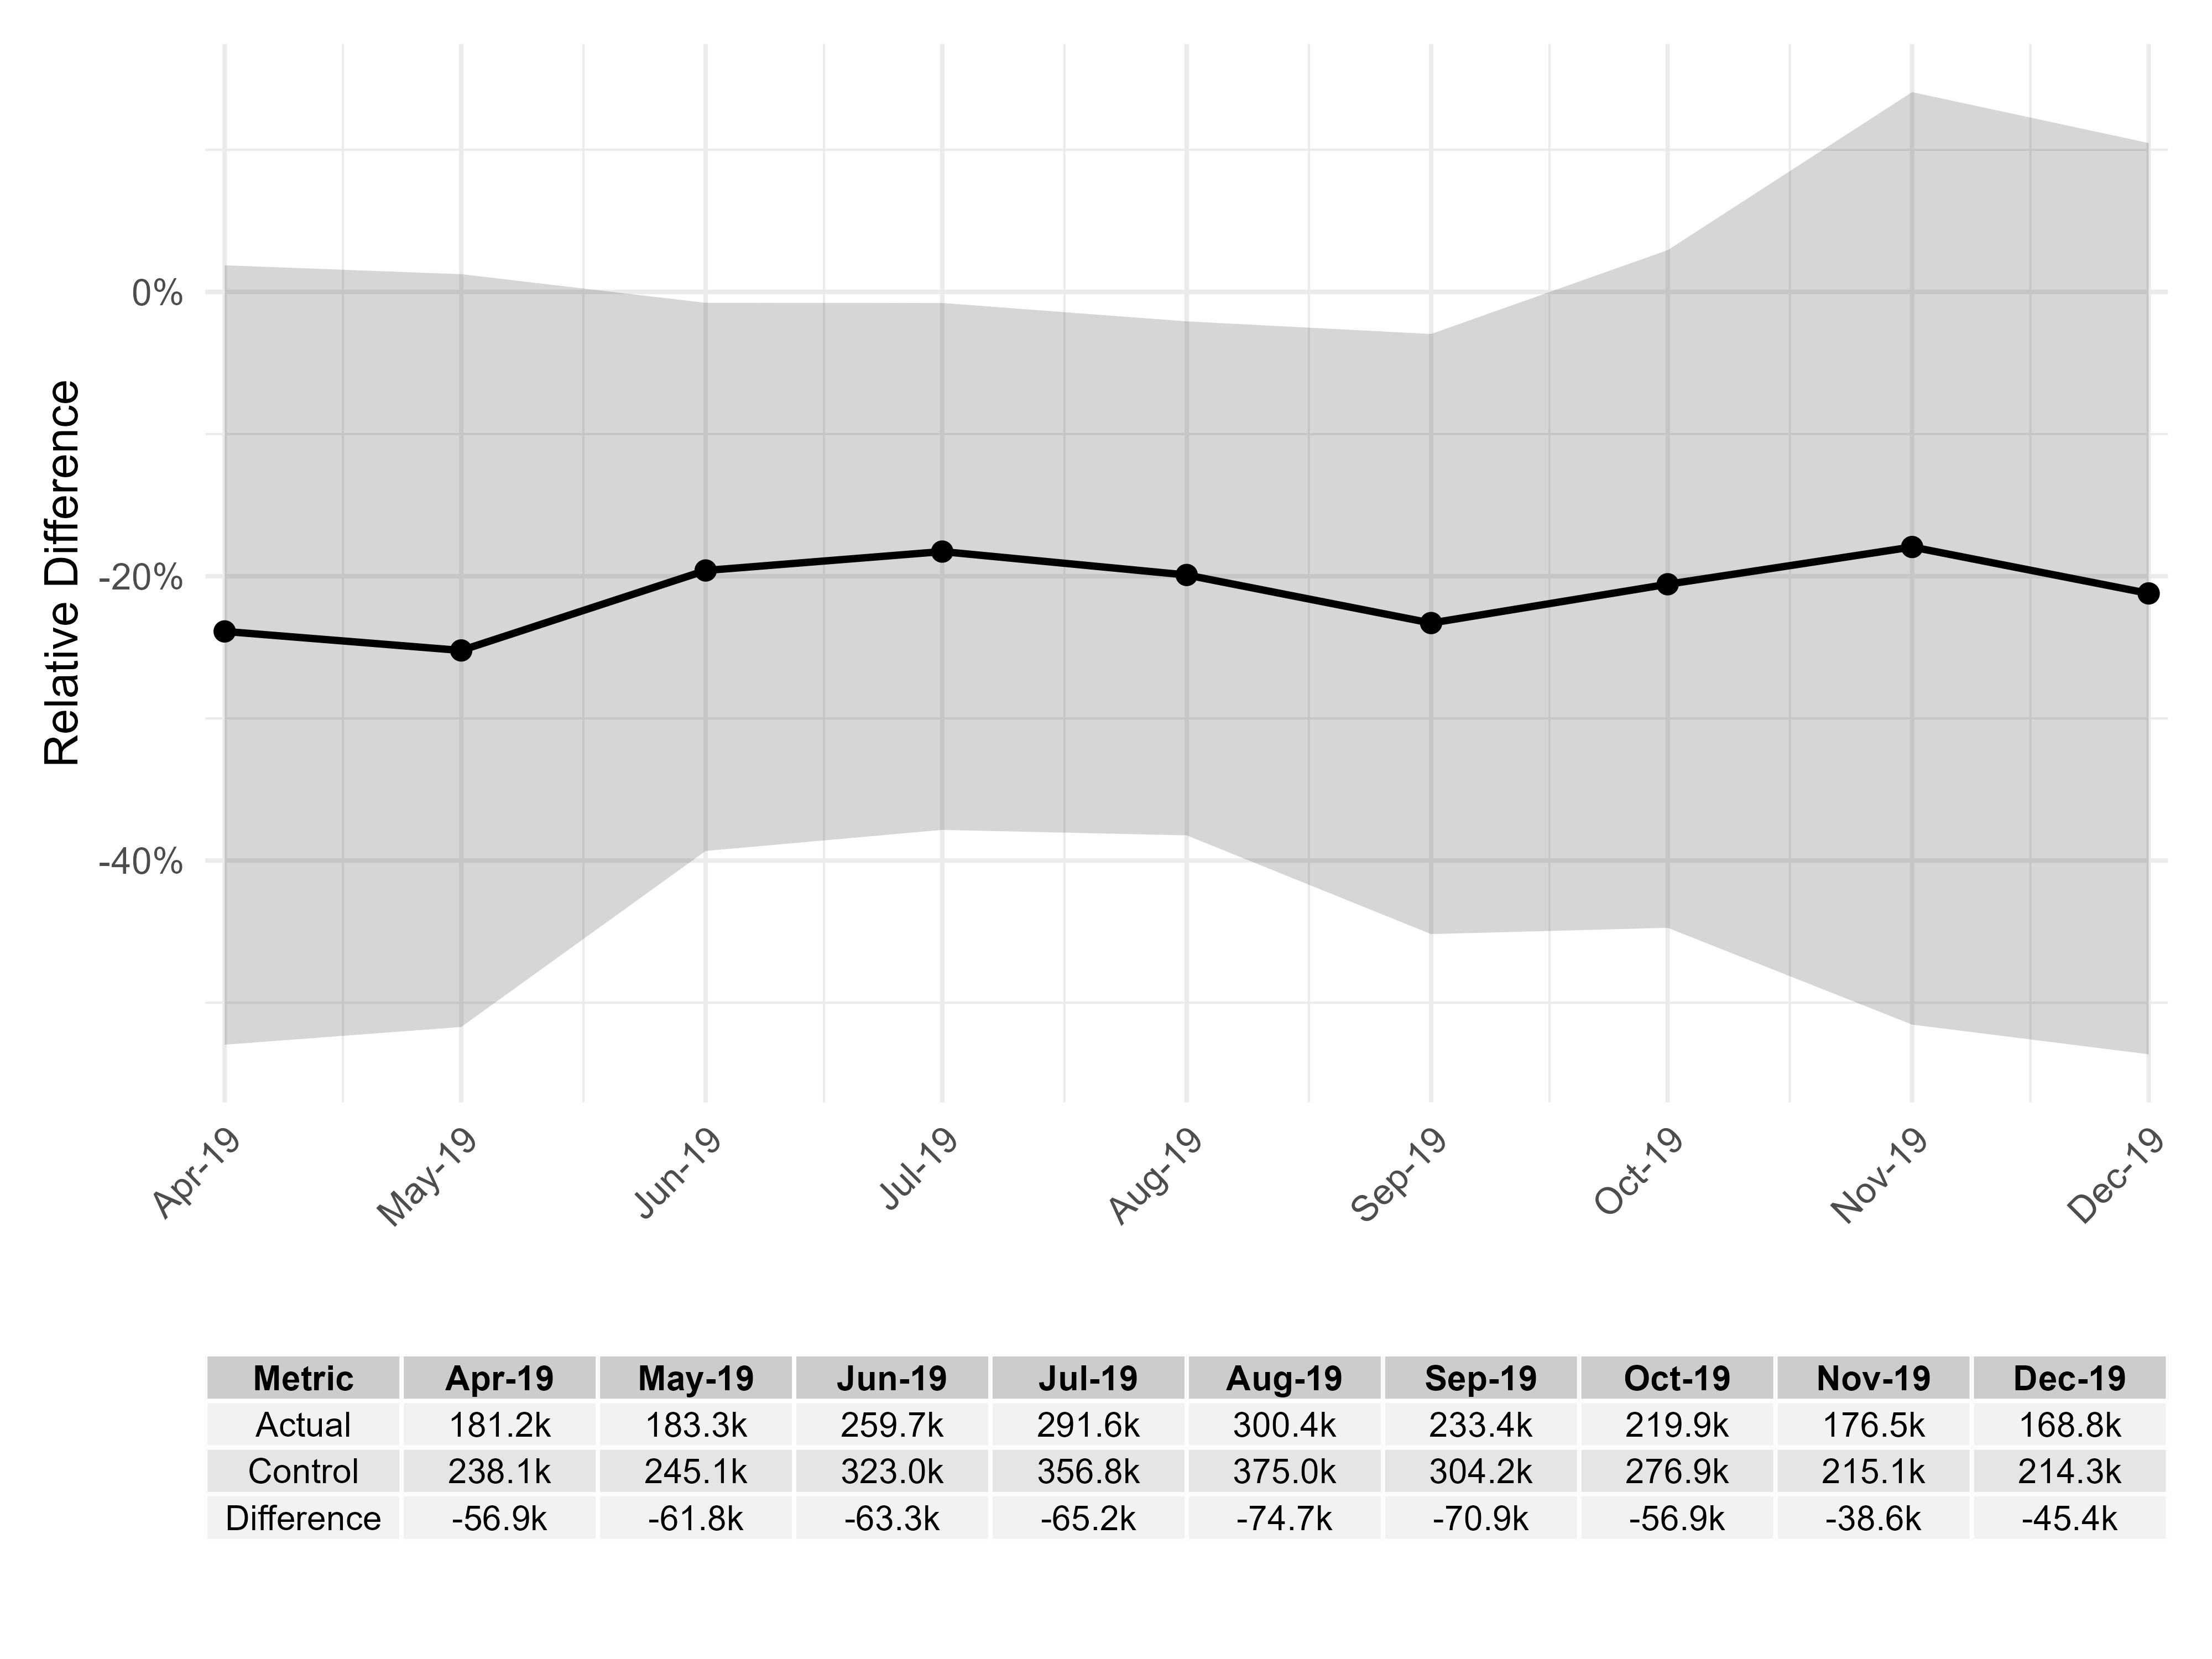
\includegraphics[width=\textwidth]{Figures/Figure 6.jpg}
\begin{minipage}{\textwidth}
\footnotesize \tiny \textit{Note:} The solid line shows the estimated monthly percentage difference between observed and counterfactual departures. Shaded areas represent 95\% credible intervals from the Bayesian structural time series model. The table below reports actual, predicted, and difference values for each month.
\end{minipage}
\label{fig:monthly_diff_plot}
\end{figure}


Because subsequent results build directly on the finding that tourism supply was substantially affected by the bankruptcy and because I utilize the same model and calibration for remaining outcomes, it is essential that this estimate be robust and credible. To this end, I implement a broad set of placebo and specification checks, detailed in the Appendix. Placebo tests apply the same treatment to outcomes or countries that should be unaffected, providing a check against false positives and helping guard against type I error. These include assigning the bankruptcy shock to other Nordic countries, to unrelated Icelandic outcomes such as fish landings, and to pre-bankruptcy periods. Only the pre-bankruptcy placebos show notable treatment effects, likely capturing WOW Air’s expansion rather than a true shock, though these estimates are much less precise than the true bankruptcy effect, with placebo results significant at roughly the 1\% level compared to 0.02\% (p=0.0002) for the actual bankruptcy. Robustness tests varying the control countries used, covariate information included, and model specifications all yield consistent null results, and comparison with a two-way fixed effects model shows estimates of similar magnitude, underscoring the reliability of the BSTS approach. Together, these tests reinforce confidence that the observed decline in passengers is causally attributable to the bankruptcy.

\subsection{Labor Levels}
Having shown that the closure of WOW Air resulted in a significant tourism supply shock to Iceland, we may exploit this fact to estimate the impacts to other economic indicators related to tourism and reasonably assume that the bankruptcy was the mechanism for the resulting changes. I turn to the labor market, where the consequence of the supply shock was both immediate and substantial. The following subsections trace the effects on unemployment levels at the national level, across sectors, and through resulting taxable wages, before contextualizing the magnitude of these impacts with pre-shock specialization.

\begin{figure}[htbp]
\centering
\caption{National labor impacts}
\label{fig:national_labor_grouped}
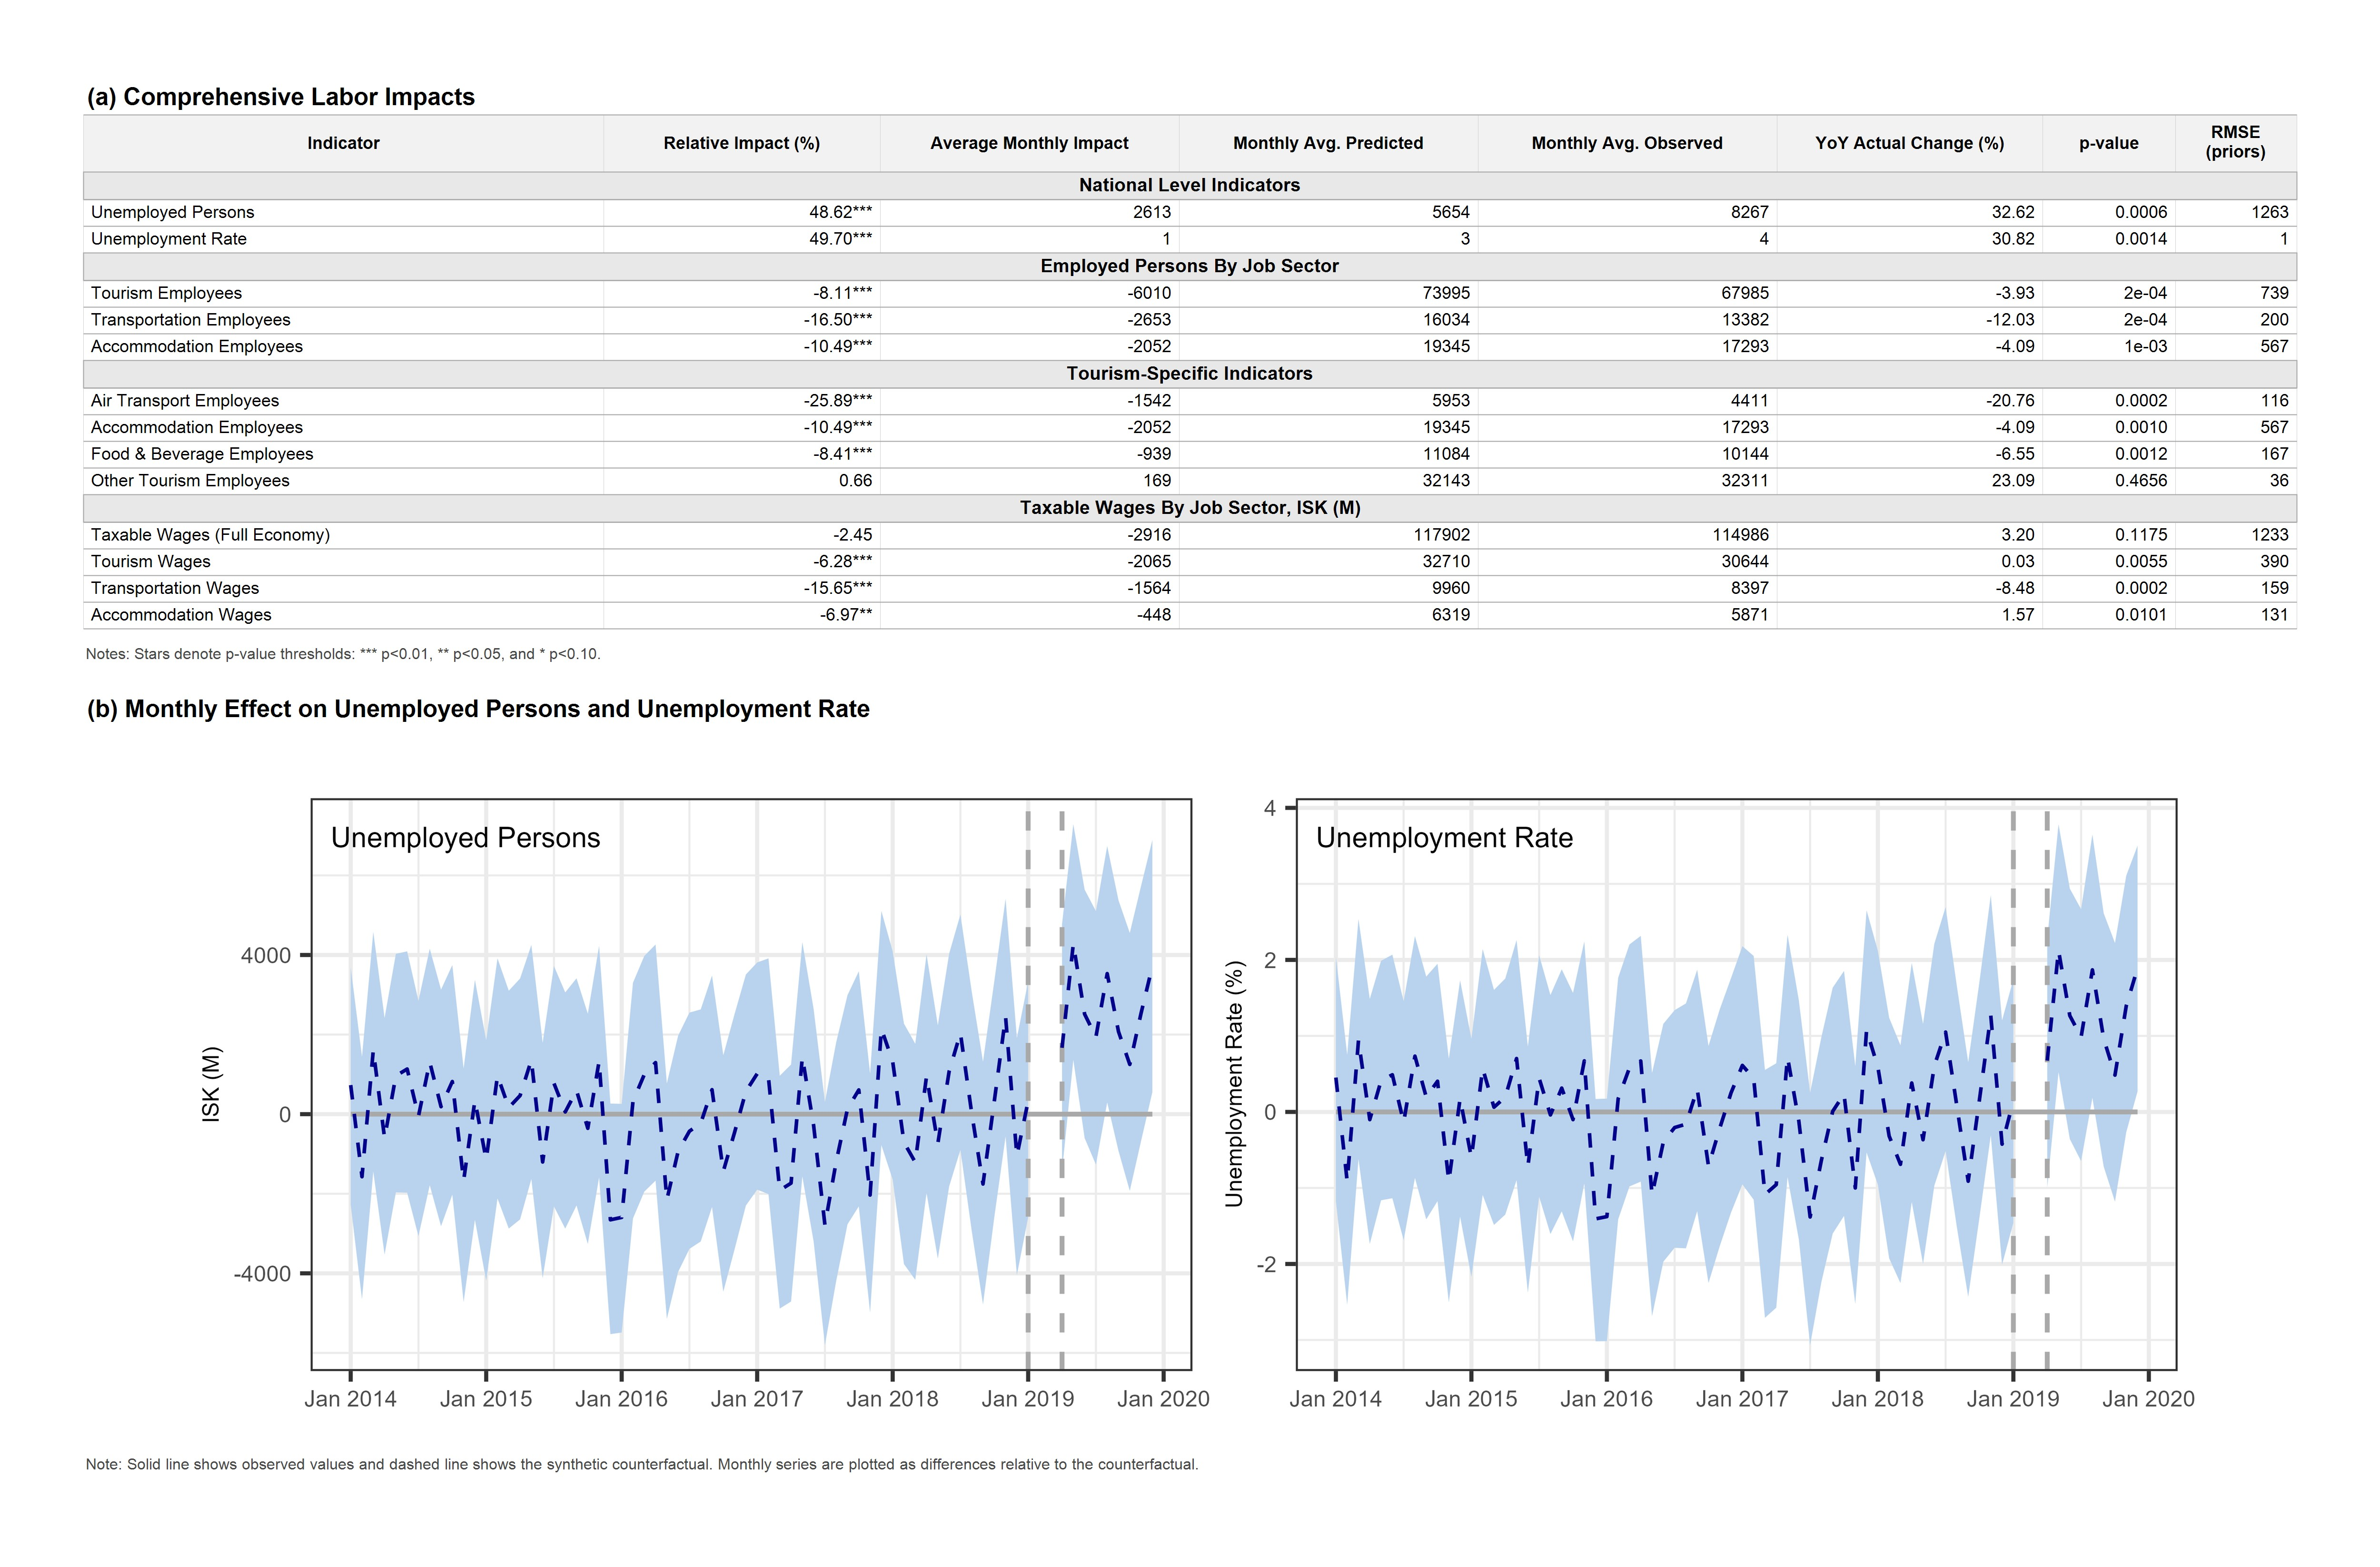
\includegraphics[width=\textwidth]{Figures/Figure 7.jpg}
\end{figure}

\paragraph{Sectoral employment effects.}
The panel Employed Persons By Job Sector in Figure \ref{fig:national_labor_grouped}a shows that overall tourism employment fell by 8.1\%, or roughly 6,000 jobs per month, relative to the counterfactual. These values represent deviations from the projected growth path rather than true job losses, likely reflecting a combination of foregone employment that would likely have occurred had pre-shock trends continued and actual jobs lost. Air transport experienced the steepest decline in employment at 25.9\% ($-1,540$ jobs), and the broader transport sector fell by 16.5\% ($-2,650$ jobs). For context, WOW Air employed between 1,000 and 1,100 workers at the time of its bankruptcy, and in the counterfactual scenario, continued growth would likely have been expected. Additional labor losses appeared in accommodation ($-10.5\%$) and food \& beverage ($-8.4\%$), though these estimates carry greater statistical uncertainty. Collectively, these results confirm that employment reductions were felt deeply within tourism-related industries.

\paragraph{National unemployment response.}
The sharp contractions in tourism-facing sectors also led to an aggregate rise in national unemployment. Figure \ref{fig:national_labor_grouped}b shows the monthly differences between actual unemployment levels and the synthetic at the national level, while the National Level Indicators panel of Figure \ref{fig:national_labor_grouped}a presents the corresponding estimated effects. The number of unemployed persons increased by 48.5\% relative to the counterfactual, equivalent to about 2,600 additional unemployed workers per month. The unemployment rate rose by 1.3 percentage points, or 49.5\% relative to the counterfactual. These are substantial shifts within a labor force of roughly 200,000 workers, yet they are substantially lower than the projected 6,000 employee decrease in tourism, indicating a likely shift across sectors. As mentioned, because this method measures differences relative to a modeled counterfactual rather than tracking actual losses. Consequently, this approach cannot test for cross-sectoral labor shifts, especially as non-tourism employment and tourism employment are likely endogenous, as the expansion of tourism can contribute to wider job creation across the economy.

Yet, when the effects of the bankruptcy on employment is measured net of tourism, the evidence becomes less precise ($p = 0.0141$). Total non-tourism employment grew relative to the counterfactual, though its composition differs. In a simpler measure, employment in tourism fell by roughly $3.9\%$ year-over-year (approximately $-4,000$ jobs), while employment outside of tourism rose by about $3.93\%$ ($+2,500$ jobs).


\paragraph{Taxable wages.}
Employment losses are also reflected in taxable wage data, though the declines are less pronounced at the national level.  The \textbf{Taxable Wages By Job Sector} panel of Table \ref{fig:fig_table_grouped}a  reveals transport wages (inclusive of air transport) fell by 15.6\% (–1.56 billion ISK monthly), while accommodation wages fell by 7.0\%. At the aggregate level, national wages fell by over 2\%, but without statistical significance. The lack of significance could reflect the small scale of tourism employment relative to national employment, or it could speak to the flexibility and substitution of hourly labor whereby employees leaving tourism find similar work quickly. Additionally, it could be reflective of unemployment benefits which may have cushioned part of the income loss.  

The magnitude of the labor market response is partly explained by Iceland’s high degree of specialization in tourism employment leading into 2019. As shown in Table \ref{tab:specialization}, the share of employees in tourism nearly doubled from 8\% in 2010 to 15\% in 2018. Sub-sectors such as accommodation (+65\%), tour services (+232\%), and air transport (+87\%) grew especially rapidly as a share of all employment. This concentration left the labor market highly exposed to a sudden contraction in arrivals. As shown, the share of employees in every one of these sub-sectors fell from 2018 into 2019. The WOW Air bankruptcy therefore not only reduced employment in directly affected sectors but also exposed the vulnerability created by the preceding decade of rapid specialization. While Iceland’s degree of tourism specialization may appear unusually high, significantly higher concentrations of tourism employment are observed elsewhere, increasing the generalizability of these results. Across the Caribbean, travel and tourism comprise a dominant share of total employment, peaking at 90.7\% in Antigua and Barbuda in 2019, while all of the ten most tourism-dependent economies surpass 50\%.\footnote{Original data from the World Travel and Tourism Council (2019). Available at: \href{https://www.weforum.org/stories/2020/08/destinations-rely-most-on-tourism-travel/}{\textit{weforum.org}}.} These parallels highlight how economies heavily reliant on tourism face amplified labor market risks during shocks to international mobility, underscoring the importance of diversification in sustaining economic resilience.

\begin{sidewaystable}[!h]
\centering
\caption{Iceland Sectoral Employment Concentration}\label{tab:specialization}

\resizebox{\textwidth}{!}{%
\centering
\begin{table}[htbp]
\centering
\caption{Labor-Market and Wage Effects of the WOW Air Bankruptcy}\label{tab:labor_impact}
\resizebox{\textwidth}{!}{%
\begin{tabular}[t]{llrrrrrr}
\toprule
Outcome & \shortstack[l]{9-Month Relative Impact (\%)\\and 95\% CI} & YoY Actual Change (\%) & Avg. Monthly Impact & Monthly Avg. Predicted & Monthly Avg. Observed & p-value & RMSE (pre-period)\\
\midrule
\multicolumn{8}{l}{\textbf{National labor indicators}}\\
Unemployed Persons & 46.21***\hspace{0.6em}[22.8, 72.3] & 32.62 & 2,613 & 5,654 & 8,267 & 0.0006 & 1,263 \\
Unemployment Rate & 46.93***\hspace{0.6em}[22.4, 73.2] & 30.82 & 1.30 & 2.76 & 4.06 & 0.0014 & 0.66 \\
\midrule
\multicolumn{8}{l}{\textbf{Employment by sector}}\\
Tourism Employees & -8.12***\hspace{0.6em}[-10.8, -5.4] & -3.93 & -6,010 & 73,995 & 67,985 & 0.0002 & 739 \\
Tourism Employees, Net of Air Transport & -6.61***\hspace{0.6em}[-9.3, -3.3] & -2.49 & -4,498 & 68,072 & 63,574 & 0.0010 & 765 \\
Transportation Employees & -16.54***\hspace{0.6em}[-20.6, -12.6] & -12.03 & -2,653 & 16,034 & 13,382 & 0.0002 & 200 \\
Transportation Employees, Net of Air Transport & -11.94***\hspace{0.6em}[-16.2, -6.7] & -6.99 & -1,217 & 10,187 & 8,971 & 0.0002 & 162 \\
Accommodation Employees & -10.61***\hspace{0.6em}[-15.3, -4.9] & -4.09 & -2,052 & 19,345 & 17,293 & 0.0010 & 567 \\
Air Transport Employees & -25.90***\hspace{0.6em}[-31.0, -20.9] & -20.76 & -1,542 & 5,953 & 4,411 & 0.0002 & 116 \\
Food \& Beverage Employees & -8.47***\hspace{0.6em}[-13.9, -3.2] & -6.55 & -939 & 11,084 & 10,144 & 0.0002 & 167 \\
Other Tourism Employees & 0.53\hspace{0.6em}[-8.3, 9.4] & 23.09 & 169 & 32,143 & 32,311 & 0.4539 & 36 \\
\midrule
\multicolumn{8}{l}{\textbf{Taxable wages by sector}}\\
Taxable Wages, Full Economy & -2.47\hspace{0.6em}[-6.5, 1.8] & 3.20 & -2,916 & 117,902 & 114,986 & 0.1175 & 1,233 \\
Tourism Wages & -6.31***\hspace{0.6em}[-11.5, -1.6] & 0.03 & -2,065 & 32,710 & 30,644 & 0.0042 & 390 \\
Transportation Wages & -15.70***\hspace{0.6em}[-21.5, -9.6] & -8.48 & -1,564 & 9,960 & 8,397 & 0.0002 & 159 \\
Accommodation Wages & -7.08***\hspace{0.6em}[-12.7, -1.2] & 1.57 & -448 & 6,319 & 5,871 & 0.0075 & 131 \\
\bottomrule
\end{tabular}
}
\begin{minipage}{\textwidth}
\raggedright\scriptsize \textit{Note:} Relative impact and its 95\% interval compare cumulative observed and counterfactual outcomes over April--December 2019. YoY actual change compares the observed nine-month average with the same months of 2018. Monthly quantities and RMSE are measured in workers for employment and unemployment, percentage points for the unemployment rate, and ISK millions for wages. Stars denote statistical significance: *** $p<0.01$, ** $p<0.05$, * $p<0.10$.
\end{minipage}
\end{table}

  }
  \begin{tablenotes}
    \footnotesize
\item \textit{Note:} Values are calculated using monthly data aggregated to annual averages. Percentage changes are computed using annual averages and reflect relative growth between periods. 
\end{tablenotes}
\end{sidewaystable}

\begin{figure}[h]
    \caption{Monthly Differences in Estimated and Realized Labor Levels}
\centering
    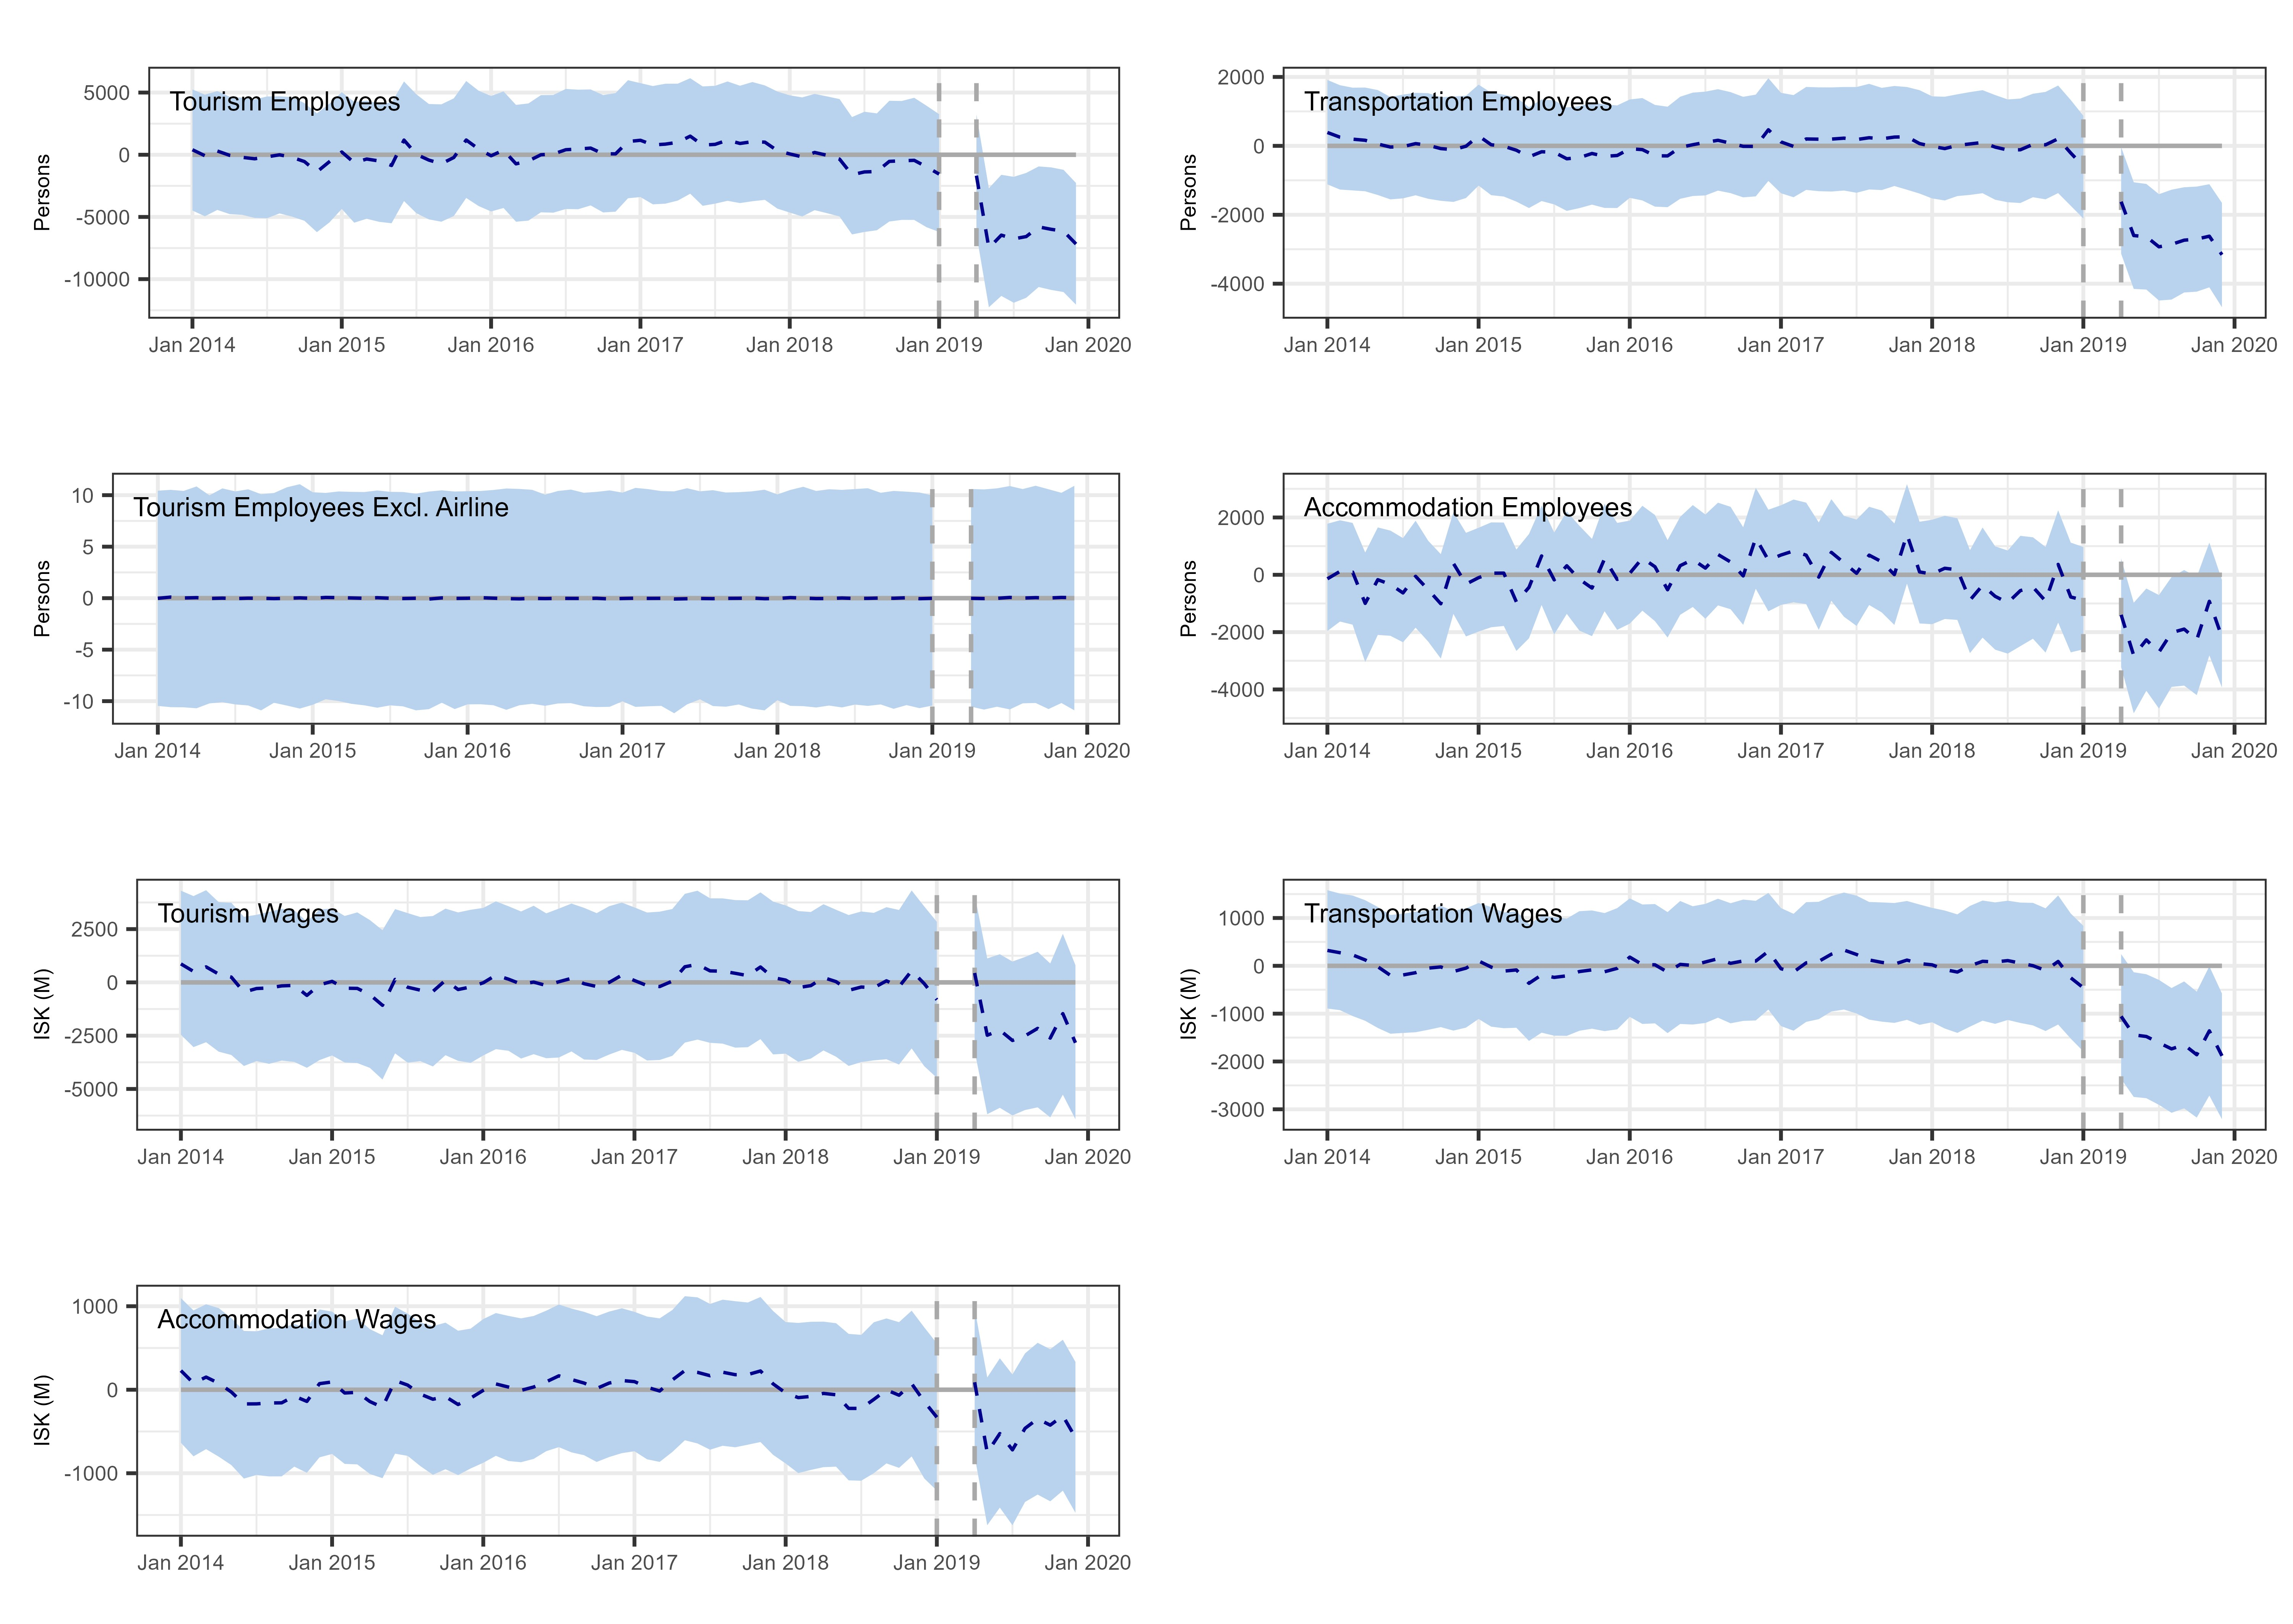
\includegraphics[width=1\textwidth, height=0.5\textheight]{Figures/Figure 8.jpg}\
\begin{minipage}{\textwidth}
\footnotesize \textit{Note:} The dashed line shows the difference between the synthetic counterfactual and the observed; shaded areas indicate uncertainty.
\end{minipage}
\label{fig:Sectoral Impact Plot}
\end{figure}

\section{Conclusion}\label{sec:conclusion}
The collapse of WOW Air illustrates how a seemingly narrow, firm-specific event can trigger broader economic disruptions in a small, tourism-dependent economy. The shock spread quickly through the labor market, with consequences significant enough to be visible in aggregate national indicators.  

That WOW Air was a low-cost carrier is particularly notable. Although often viewed as peripheral, such carriers can underpin large volumes of activity by creating new routes and demand that are not easily replaced when withdrawn. This case shows that their exit can reverberate widely, affecting employment, fiscal revenues, and economic stability.  

Beyond documenting realized vulnerability, the study contributes causal evidence to a literature often limited to descriptive indices or correlations between tourism and growth. It highlights how quickly international travel shocks can translate into labor market dislocations and fiscal pressures, underscoring the importance for policymakers of recognizing the risks of over-specialization, strengthening resilience planning, and considering targeted support mechanisms for economies reliant on sustained visitor inflows. Further, we demonstrate that there is opportunity to help mitigate a hard bankruptcy and to support the anticipated employment losses in tourism sub-sectors across the region.

% The appendix command is issued once, prior to all appendices, if any.
\section{Appendix}\label{sec:Appendix}
\subsection{Placebo Checks}\label{sec:appendix_placebos}
An advantage of the Bayesian Structural Time Series approach is that it can easily be directly tested for accuracy through placebo exercises. These tests provide evidence on the model’s ability to avoid Type II error and help identify potential limitations in specification. I present three categories of placebo checks: (1) treatment on an unrelated industry, (2) treatment applied to an untreated country, and (3) treatment applied to years prior to the bankruptcy. Model calibration is identical to our primary model, except as otherwise noted. The full set of results is summarized in Table \ref{tab:complete_placebo_panel}, with further discussion below.


\begin{sidewaystable}[htbp]
  \caption{Placebo Counterfactual Analysis}\label{tab:complete_placebo_panel}
\resizebox{\textwidth}{!}{%
\centering
  \begin{tabular}[t]{lrrrrrr}
\toprule
Indicator & Relative Impact (\%) & 9-Month Cumulative Impact & 95\% CI Upper & 95\% CI Lower & p-value & RMSE (priors)\\
\midrule
Total Passengers & -20.63*** & -533,643 & -251,386 & -942,546 & 0.0002 & 13,530\\
Icelandic Passengers & -16.70*** & -100,771 & -23,111 & -180,957 & 0.0010 & 2,905\\
Foreign Passengers & -22.75*** & -461,168 & -211,729 & -831,090 & 0.0002 & 11,895\\
\midrule
Fish Landings & -2.85 & -32,226,026 & 130,028,394 & -186,611,760 & 0.3332 & 23,174,309\\
\midrule
Greenland & -0.06 & -1,888 & 20,564 & -25,954 & 0.4367 & 229\\
Faroe Islands & 9.03 & 23,269 & 69,160 & -32,872 & 0.1381 & NA\\
Denmark & -3.22 & -449 & 414 & -1,275 & 0.1622 & 41\\
Norway & 1.88 & 166,696 & 736,165 & -520,793 & 0.2666 & 21,952\\
\midrule
Impact in January 2018 & -7.49* & -198,384 & 75,442 & -448,867 & 0.0726 & 11,081\\
Impact in January 2017 & 8.43 & 146,501 & 490,215 & -431,687 & 0.2428 & 11,023\\
\bottomrule
\end{tabular}

  }
  \begin{tablenotes}
    \footnotesize
    \item \textit{Note:} Reported measures by country showing variation in availability and level of detail across topic areas.
  \end{tablenotes}
\end{sidewaystable}

\subsubsection{Treatment on Unrelated Industry}\label{sec:Placebo1}

Applying the bankruptcy shock to the weight of fish landings yields no statistically significant effect (Table \ref{tab:complete_placebo_panel}, Panel Impact of Bankruptcy on Fish Landing Weight). This confirms that the model does not spuriously generate effects in sectors unrelated to international air travel. In practical terms, this indicates that the observed results are not simply an artifact of how the model fits time-series data, but are specific to sectors plausibly affected by air transport disruptions.

\subsubsection{Treatment on Untreated Country}\label{sec:Placebo2}

Placebo treatments applied to control countries show that the estimated impacts are not replicable outside of Iceland (Table \ref{tab:complete_placebo_panel}, Panel Impact of Bankruptcy on Other Countries). When the 2019 bankruptcy shock is imposed on Greenland, Denmark, or Norway, the resulting impacts are small in magnitude and statistically insignificant. The Faroe Islands is not significant, but is large in magnitude with an estimated relative effect of around +9\%. However, given the small scale of the Faroese economy, this is likely attributable to data volatility rather than a genuine treatment effect. These findings reinforce that the large and persistent decline in Icelandic passenger volumes is not detected in the untreated nations, as expected.

\subsubsection{Treatment Years Prior}\label{sec:Placebo3}

When the bankruptcy shock is assigned to earlier years (2017 or 2018), the model detects a marginally statistically significant negative effect for the year 2018 (Table \ref{tab:complete_placebo_panel}, Panel Impact of 2019 Bankruptcy on Iceland for Years Prior). This may reflect an overall cooling of the tourism sector, or perhaps an anticipatory contraction in WOW Air flights, in an effort to avoid bankruptcy. While such findings suggest a potential cooling of the tourism sector prior to 2019, the strength of statistical support differs markedly: placebo effects in earlier years are detected at the 5–10\% significance level, whereas the actual 2019 bankruptcy effect is identified at $p = 0.0002$, representing an effect roughly 350 times times more statistically significant than those observed in earlier periods ($p = 0.07$). This contrast provides further evidence that the observed impacts in 2019 represent a true disruption rather than a modeling artifact. Furthermore, if there was a cooling of tourism demand in 2018, that change in trend is included in the 2019 iteration. To address remaining concerns over time trends, I also present in the Appendix two alternative specifications of the time dynamics, both of which continue to yield a significant estimated impact of the bankruptcy on Icelandic tourism.

\subsection{Robustness Checks}\label{sec:Robustness}
Another advantage of the Bayesian Structural Time Series (BSTS) model is its flexibility and the ability to test robustness through alternative specifications. Because there are seemingly limitless combinations of model calibrations, I focus on the main finding - predicted total departures from Iceland - and present three robustness exercises: (1) varying the choice of control countries, (2) varying the set of covariates, and (3) estimating a counterfactual without time-series components. We can consider these a test of Type 1 Error. Across all tests, the estimated passenger loss remains large and significant, providing confidence in the primary results.  

\subsubsection{Control Country Selection}\label{sec:robustness1}
First, I vary the set of control countries to ensure that results are not driven by over-specification, or by idiosyncratic behavior in a self-selected control group. Across alternative combinations of Greenland, Faroe Islands, Denmark, and Norway, the estimated relative impact remains between –20.3\% and –28.8\%, with p-values below 0.0002 for all specifications. This suggests the results are not sensitive to which countries are included as controls. See Table \ref{tab:choice_control_Countries}. 


\begin{table}
\caption{Choice of Control Countries}
\label{tab:choice_control_Countries}
\centering
  \resizebox{\textwidth}{!}{%
  \begin{table}

\caption{Choice of Control Countries}
\centering
\begin{tabular}[t]{l|l|r|r|r|r|r}
\hline
Omitted Control Country & Relative Impact (\%) & 9-Month Cumulative Impact & 95\% CI Upper & 95\% CI Lower & p-value & RMSE (priors)\\
\hline
Greenland & -20.76*** & -541088 & -242333 & -949894 & 2e-04 & 13870\\
\hline
Faroe Islands & -22.25*** & -592873 & -272968 & -1086378 & 2e-04 & 12945\\
\hline
Denmark & -28.00*** & -791612 & -475845 & -1101349 & 2e-04 & 19983\\
\hline
Norway & -20.32*** & -531946 & -219361 & -1012257 & 4e-04 & 14075\\
\hline
Faroe Islands \& Greenland & -21.48*** & -561587 & -255975 & -950749 & 2e-04 & 13839\\
\hline
Greenland \& Denmark & -28.74*** & -820965 & -536828 & -1112876 & 2e-04 & 20322\\
\hline
Denmark \& Faroe Islands & -21.00*** & -545757 & -275384 & -811216 & 4e-04 & 22257\\
\hline
Denmark \& Norway & -26.24*** & -727234 & -414095 & -1024287 & 2e-04 & 23640\\
\hline
Norway \& Faroe Islands & -20.96*** & -552702 & -219998 & -1006906 & 2e-04 & 13780\\
\hline
Mean & -23.31*** & -629529 & -323643 & -1006212 & 2e-04 & 17190\\
\hline
\end{tabular}
\end{table}

}
  \begin{tablenotes}
    \footnotesize
    \item \textit{Note:} The number of stars denotes the significance level of the coefficient estimates based on p-values, where *** indicates $p<0.01$, ** indicates $p<0.05$, and * indicates $p<0.10$.
  \end{tablenotes}
\end{table}


\subsubsection{Covariate Grouping Selection}\label{sec:robustness2}

Second, I test whether results depend on the grouping of covariates. Referring back to Table \ref{tab:information_asymmetry}, I estimate the model using only tourism-related indicators, and compare it with specifications that include alternative groupings such as transport, wages, or other economic indicators. As shown in Table \ref{tab:choice_control_coeffs}, estimated impacts range from –17.5\% to –23.6\% regardless of grouping. Extreme values are associated with lower prior fit (higher RMSE), reinforcing the choice to use tourism indicators in the main specification.  



\begin{table}
\caption{Projected Change in Tourism From Different Coefficient Groups}
\label{tab:choice_control_coeffs}
\centering
\resizebox{\textwidth}{!}{
<<<<<<< Updated upstream
\begin{tabular}[t]{l|r|r|r|r|r|r}
\hline
Indicator & Relative Impact (\%) & 9-Month Cumulative Impact & 95\% CI Upper & 95\% CI Lower & p-value & RMSE (priors)\\
\hline
Registered Rental Vehicles & -16.97 & -46414 & -17085 & -71118 & 0.0004 & 1020\\
\hline
Total Fuel Purchases (at Pump) & -10.26 & -26555 & -767 & -58182 & 0.0219 & 1037\\
\hline
Foreign Fuel Purcahses (at Pump) & -22.92 & -12764 & -1685 & -23213 & 0.0109 & 368\\
\hline
Local Fuel Purchases (at Pump) & -10.05 & -20814 & -1695 & -36779 & 0.0181 & 828\\
=======
\begin{tabular}[t]{l|l|r|r|r|r|r}
\hline
Indicator & Relative Impact (\%) & 9-Month Cumulative Impact & 95\% CI Upper & 95\% CI Lower & p-value & RMSE (priors)\\
\hline
All Indicators & -22.31*** & -583478 & -362014 & -797221 & 2e-04 & 11422\\
\hline
Passenger Indicators & -17.55*** & -435721 & -208453 & -709449 & 2e-04 & 15277\\
\hline
Tourism Indicators & -20.57*** & -533643 & -244700 & -948301 & 4e-04 & 13530\\
\hline
Labor Indicators & -22.17*** & -578100 & -359551 & -793050 & 2e-04 & 11089\\
\hline
Other Indicators & -23.63*** & -630521 & -353851 & -908255 & 2e-04 & 26532\\
\hline
Mean & -21.25*** & -552293 & -305714 & -831255 & 2e-04 & 15570\\
>>>>>>> Stashed changes
\hline
\end{tabular}
}
  \begin{tablenotes}
    \footnotesize
    \item \textit{Note:} The number of stars denotes the significance level of the coefficient estimates based on p-values, where *** indicates $p<0.01$, ** indicates $p<0.05$, and * indicates $p<0.10$.
  \end{tablenotes}
\end{table}




\subsubsection{Counterfactual Without Time-Series Components}\label{sec:robustnes3}

Finally, I estimate a simplified specification that removes all time-series and seasonality components, leaving an OLS-style regression similar to dynamic regressions proposed by \citet{banerjee_2007_modeling}. Using this approach we are predicting the outcome based solely off the relationship of the outcome variable with indicators in the control countries. 

The simplified ordinary least squares (OLS) model abstracts from the time-series dynamics of the Bayesian specification by omitting the latent level $(\mu_t)$ and seasonal $(\tau_t)$ components. The counterfactual outcome for Iceland is therefore modeled as:
\[
Y_t = \beta_0 + \sum_{j \in \mathcal{J}} x_{j,t}\beta_j + \varepsilon_t, \quad j \neq i
\]
where $Y_t$ denotes the observed outcome (e.g., international passenger departures), and $x_{j,t}$ are contemporaneous covariates from unaffected countries $j \in \mathcal{J}$.

In this specification, the set of covariates $x$ is restricted to tourism-related indicators as defined in Table \ref{tab:information_asymmetry}. Monthly, cumulative, and relative differences are computed in the same manner as in the primary model. In this case, the estimated relative loss is substantially larger (about –116,000 passengers per month compared to –60,000 in the baseline), but the direction and magnitude remain consistent (See Table \ref{tab:drop_time_series}). Figures \ref{fig:ts_drop_pointwise} and \ref{fig:ts_drop_cumulative} illustrate the associated monthly and cumulative differences. While the OLS version produces systematic pre-treatment errors, this exercise confirms that the main findings are not driven solely by trend components. While the OLS version produces systematic pre-treatment errors, this exercise confirms that the main findings are not driven solely by trend components. The inclusion of the trend terms and full BSTS specification yields a substantially better fit, as the simplified model exhibits a 27\% higher Root Mean Squared Prediction Error. Furthermore, the fact that excluding these trend components produces a larger estimated effect suggests that their inclusion biases the estimated treatment effect toward zero, implying that the full model provides a more conservative estimate of the true impact.

\begin{table}[htbp]
\caption{Forecasted Impacts Without Time-Series}\label{tab:drop_time_series}
  \resizebox{\textwidth}{!}{%

\begin{tabular}{l|l|r|r|r|r|l|l|r|r|r|r|l|l|r|r|r|r|l|l|r|r|r|r|l|l|r|r|r|r|l|l|r|r|r|r}
\hline
\textbf{Model Used} & Loss Percent & Monthly Impact & Cumulative Impact & P-Value & RMSPE\\
\hline
Simple OLS Regression, Time Series Omitted & -34.01\%*** & -115,986 & -1,043,878 & 5.2e-05 & 17,204\\
\hline
BSTS Preferred Model & -10.25\%** & -2,951 & -26,555 & 2.3e-02 & 1,037\\
\hline
\end{tabular}

}
   \begin{tablenotes} \footnotesize
    \item \textit{Note:} The number of stars denotes the significance level of the coefficient estimates based on p-values, where *** indicates $p<0.01$, ** indicates $p<0.05$, and * indicates $p<0.10$.
  \end{tablenotes}
\end{table}


\begin{figure}[h]
\centering
\caption{Projected Monthly Differences (No Time-Series Elements)}
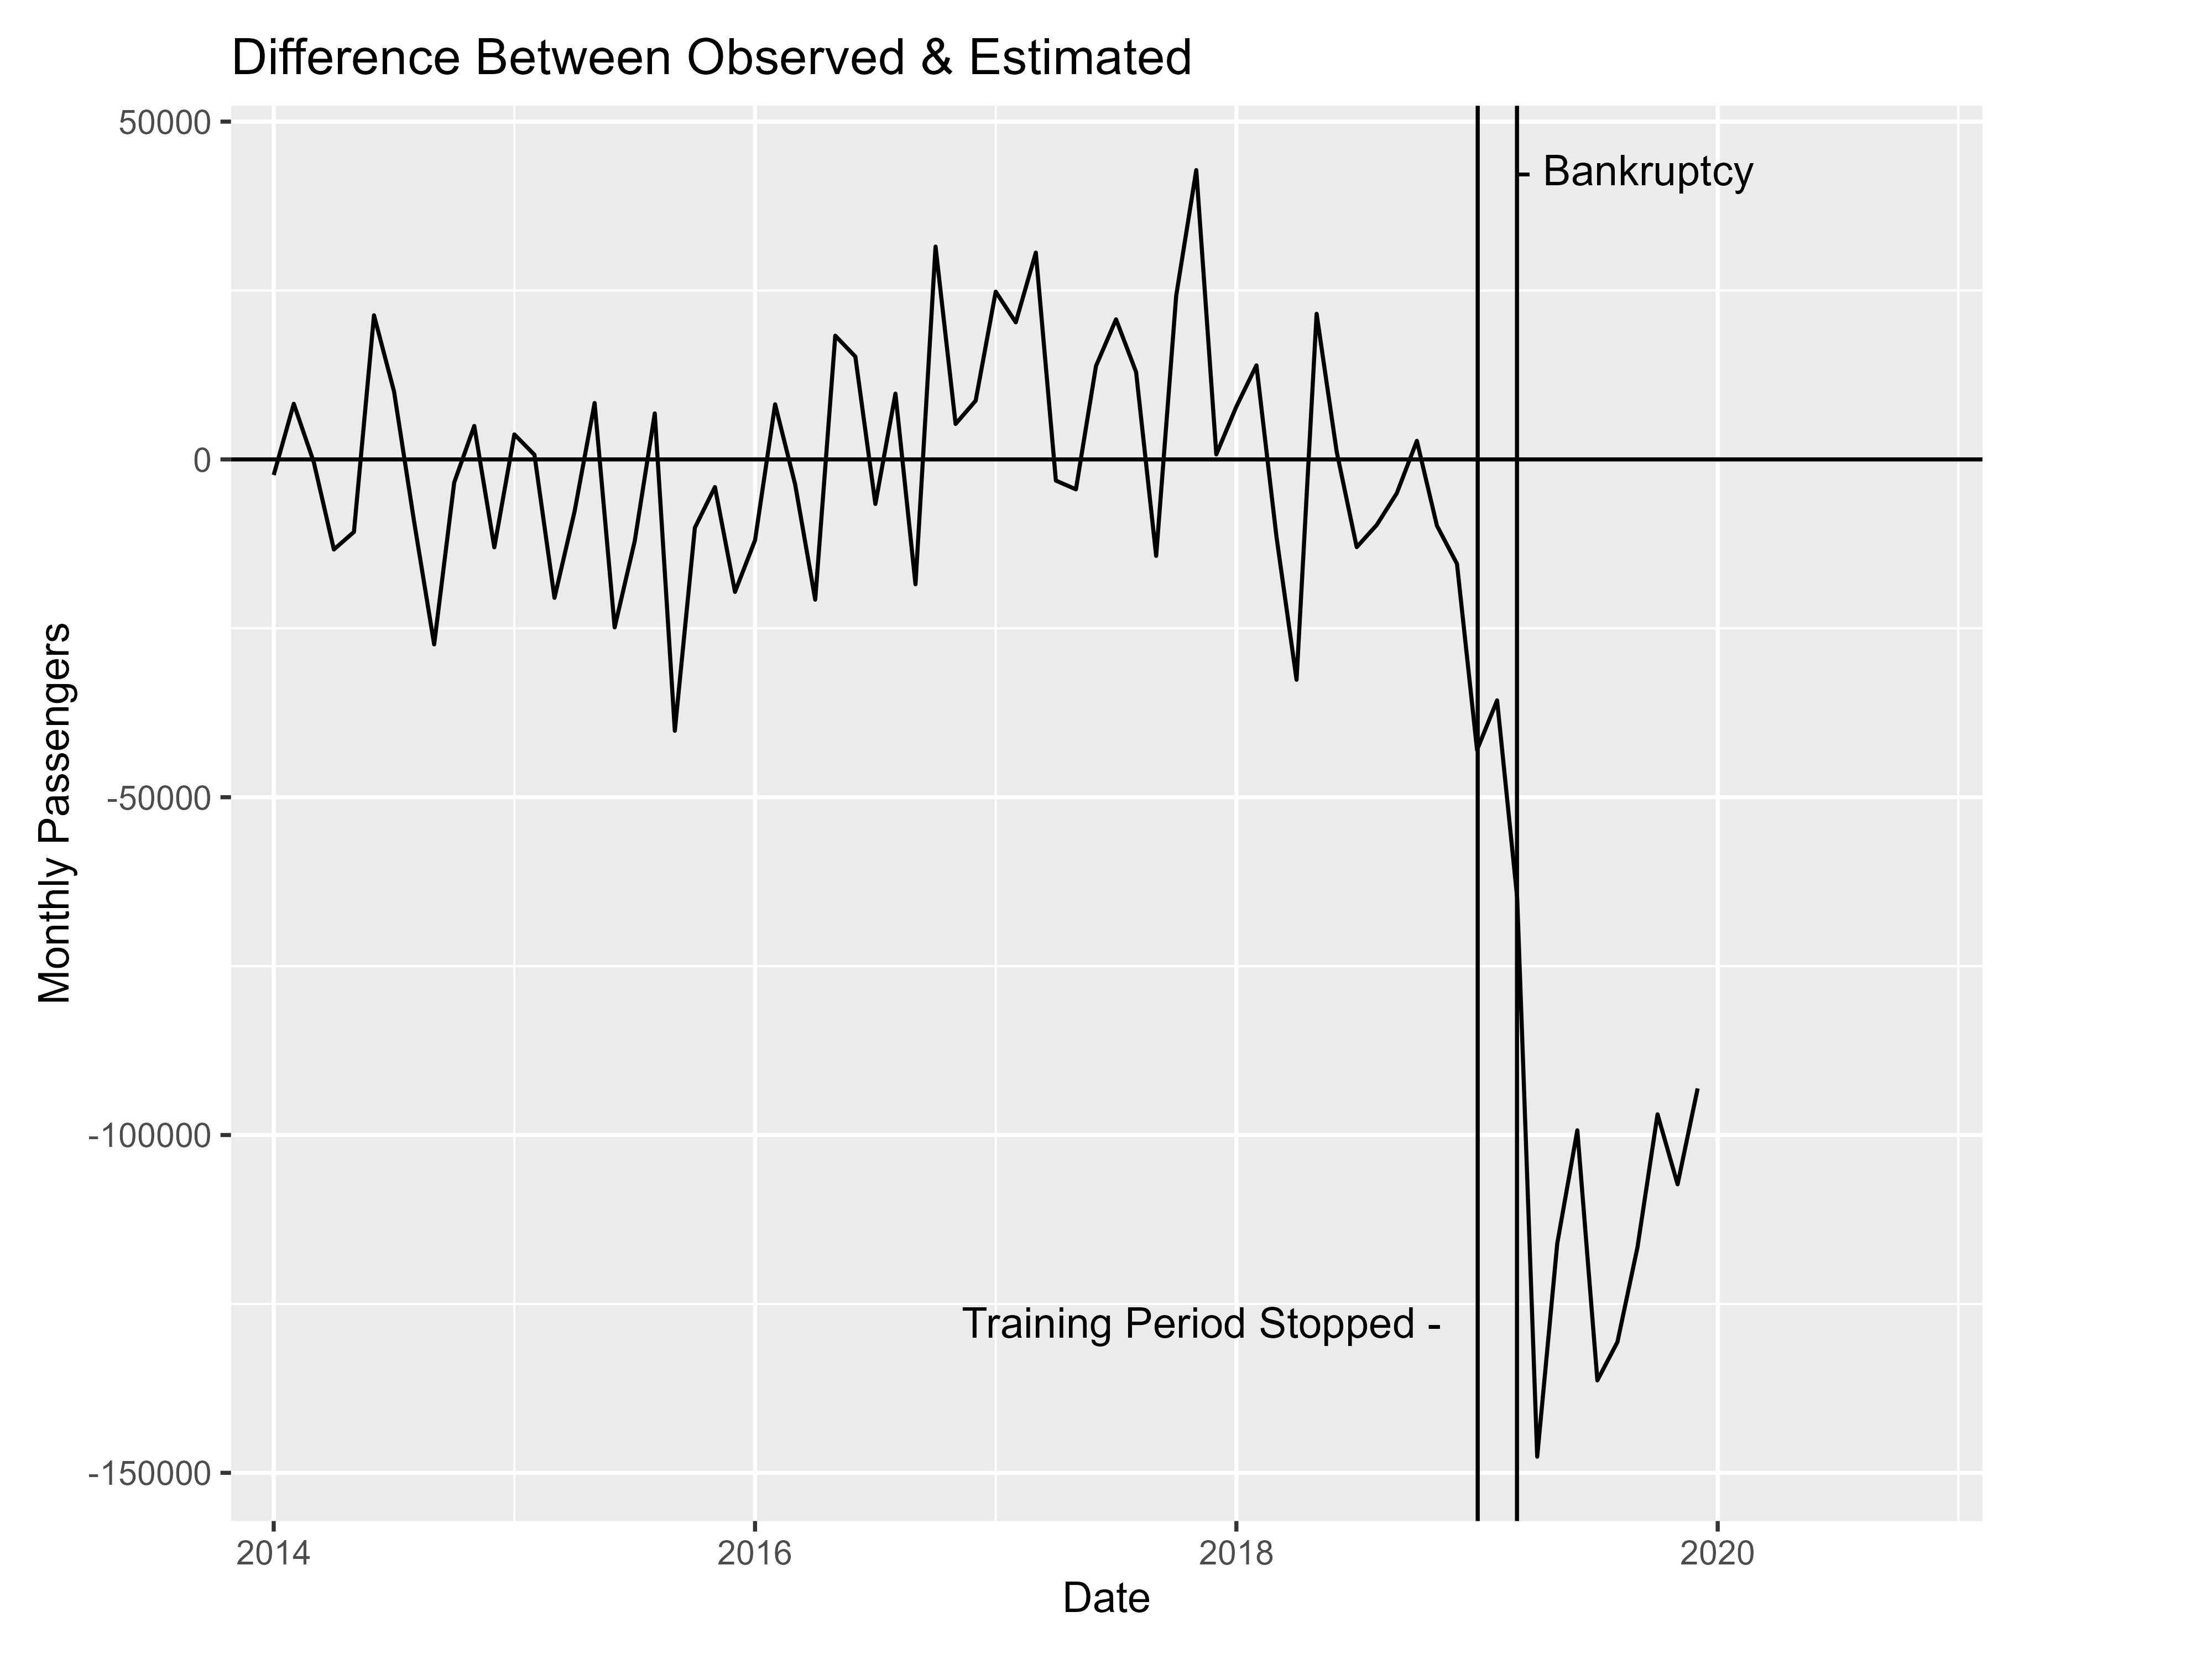
\includegraphics[width=\textwidth,height=0.7\textheight,keepaspectratio]{Figures/Figure 9.jpg}
\begin{minipage}{0.8\textwidth}
\footnotesize
\textit{Notes:} Difference between observed and estimated counterfactual monthly departures under a model without time-series elements.
\end{minipage}
\label{fig:ts_drop_pointwise}
\end{figure}

\begin{figure}[h]
\centering
\caption{Projected Cumulative Differences (No Time-Series Elements)}
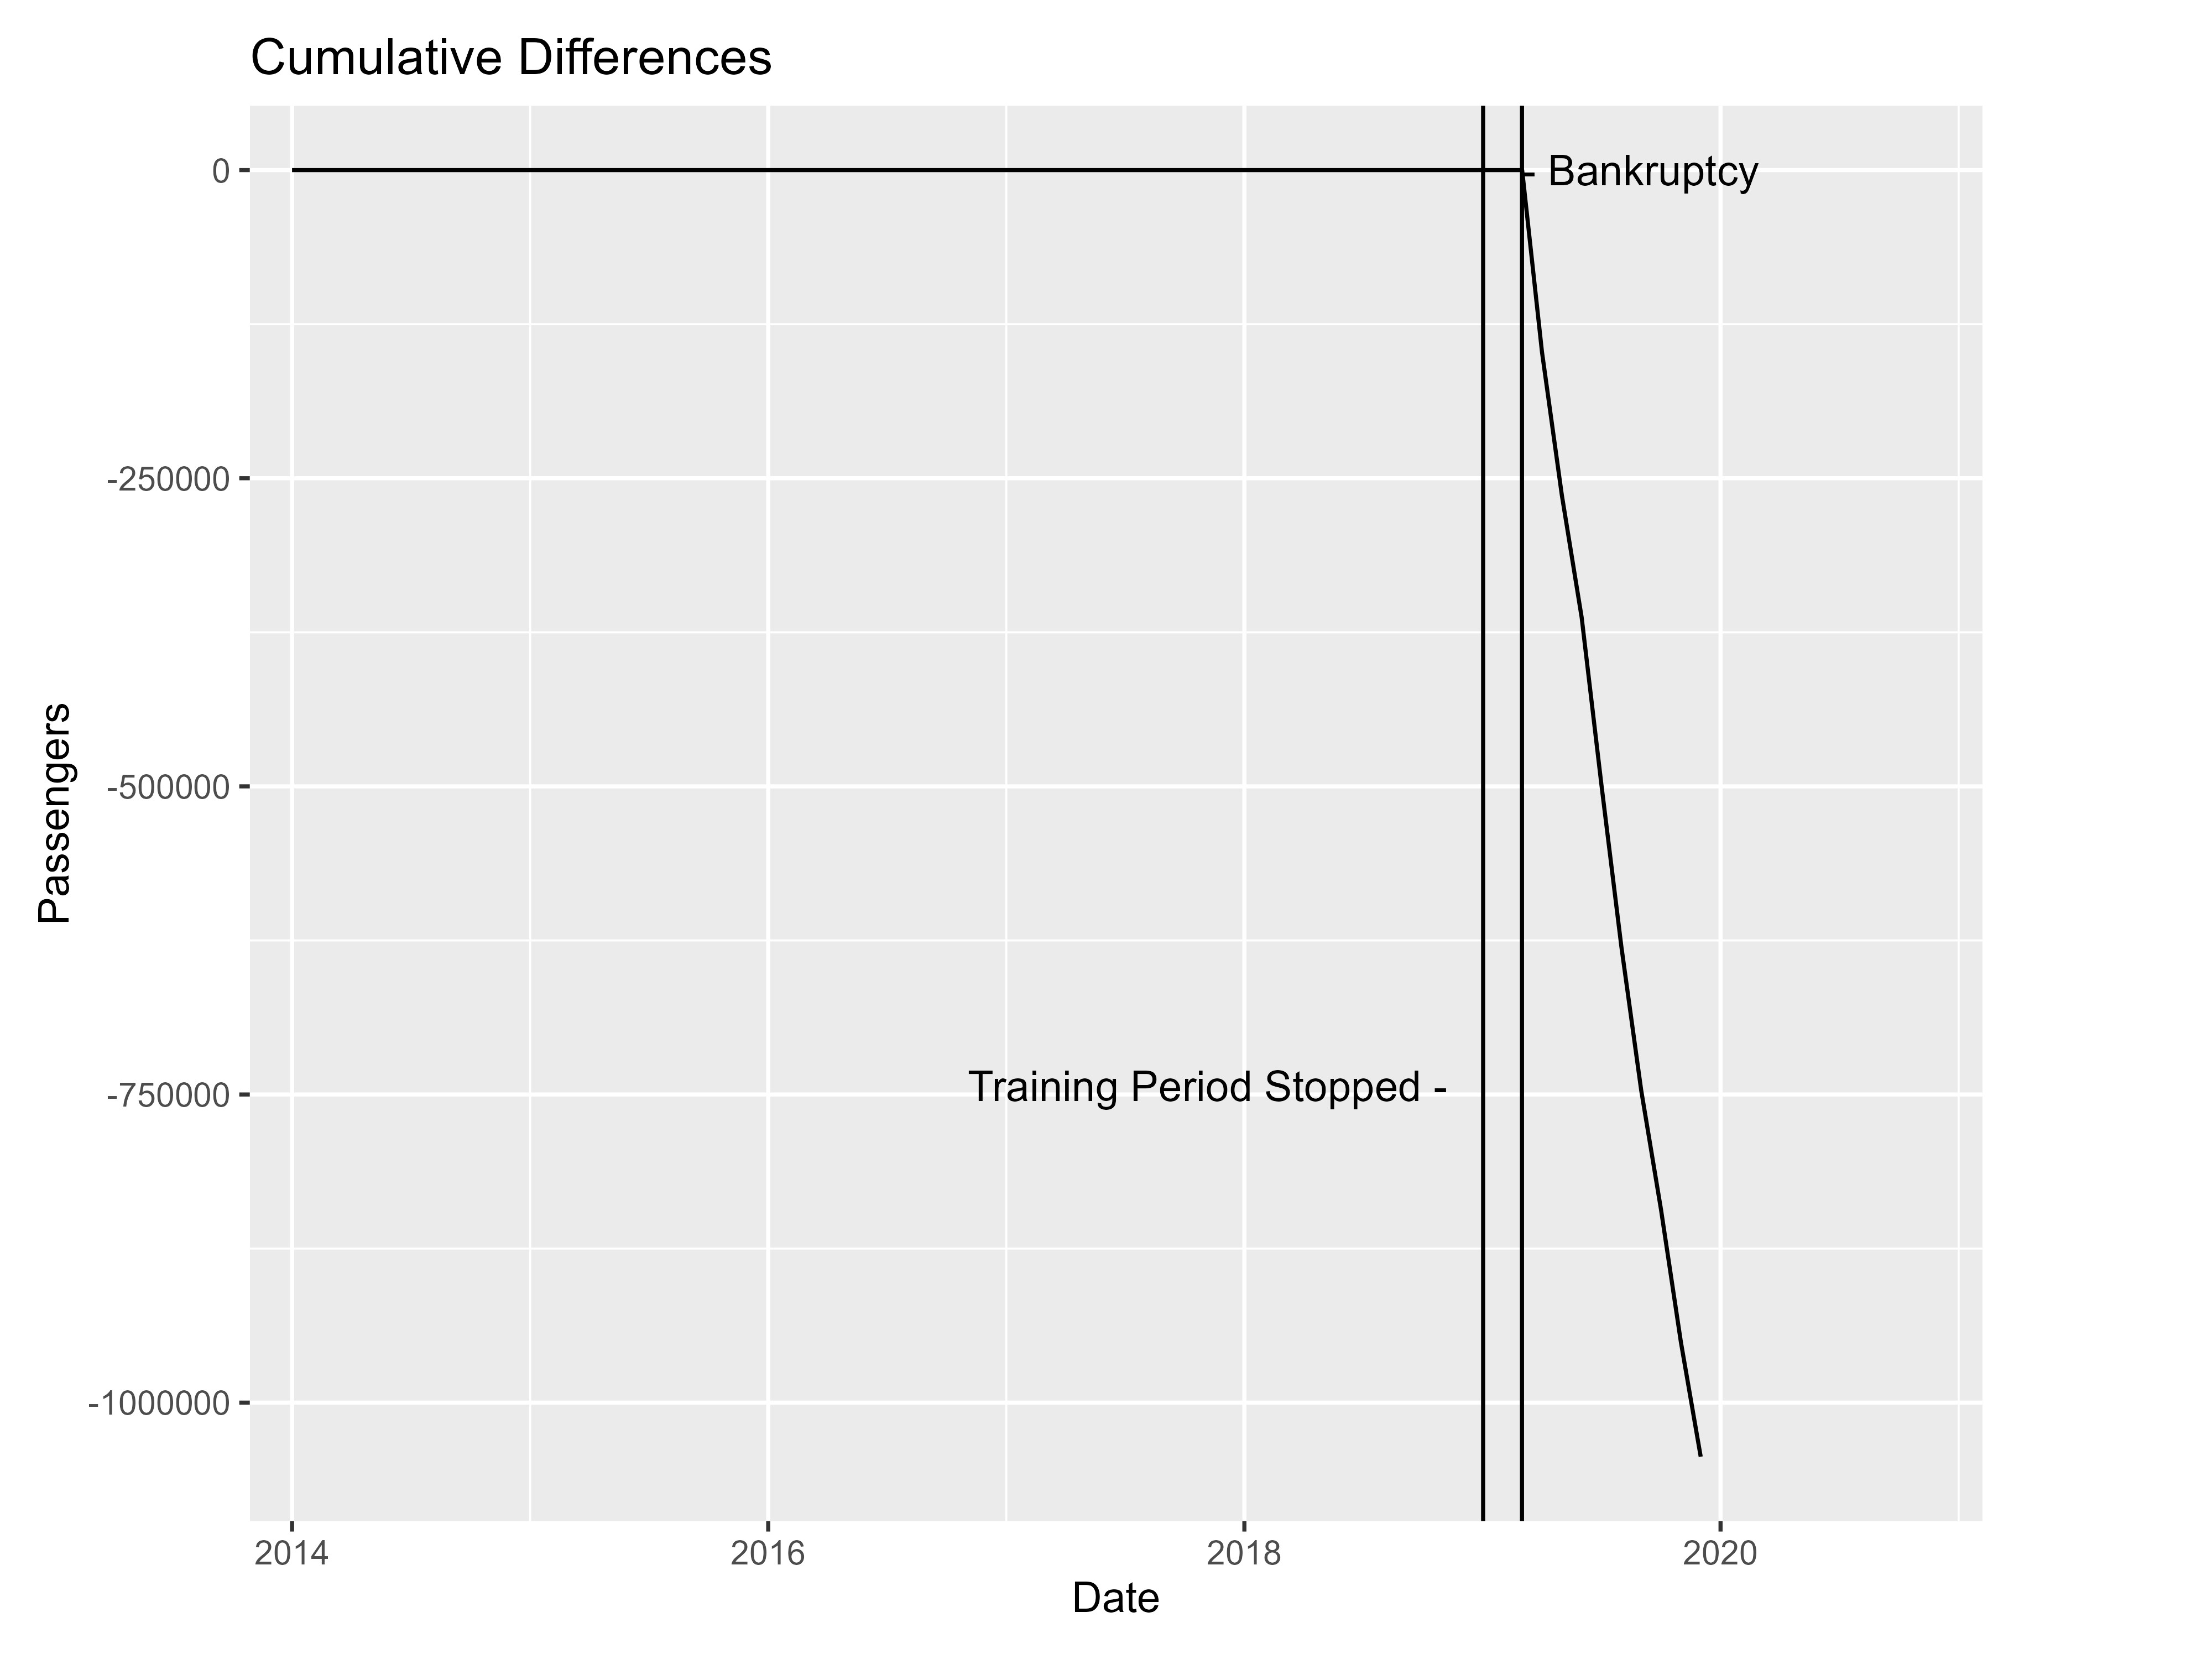
\includegraphics[width=\textwidth,height=0.7\textheight,keepaspectratio]{Figures/Figure 10.jpg}
\begin{minipage}{0.8\textwidth}
\footnotesize
\textit{Notes:} Cumulative difference between observed and estimated counterfactual departures under a model without time-series elements.
\end{minipage}
\label{fig:ts_drop_cumulative}
\end{figure}

\subsection{Two-Way Fixed Effects Comparison}\label{sec:DID_Regression}
\setlength{\parskip}{0pt}

As a benchmark, I also estimate a simple two-way fixed effects regression, while noting that the parallel trends assumption is unlikely to hold in this context. The purpose of this exercise is not to provide a definitive estimate, but rather to illustrate the limitations of a conventional Difference-in-Differences design and the relative advantages of the BSTS counterfactual. \\

The model specification is:  

\[
\begin{aligned}
\log(Y_{it}) = & \ \beta_{0} + \beta_{1} \cdot Treat_{i} + \beta_{2} \cdot (Post_{t} \times Treat_{i}) \\
& + \beta_{3} \cdot CountryFE_{i} + \beta_{4} \cdot YearFE_{t} + \beta_{5} \cdot MonthFE_{t} + \epsilon_{it}
\end{aligned}
\]

where \(Y_{it}\) is the log of arrivals for country \(i\) at time \(t\). \(Post_{t}\) is an indicator equal to 1 for the period April–December 2019 and 0 otherwise. \(Treat_{i}\) identifies exposure to the bankruptcy shock (or placebo shocks, when applied to control countries). The specification includes country, year, and month fixed effects. \\

To explore sensitivity to the pre-intervention window, I estimate this model with varying lengths of pre-period data (Table \ref{tab:DID}). Results are unstable: as additional pre-period years are included, the estimated treatment effect for Iceland not only declines in magnitude but becomes positive. When applied as placebos to the four control countries, the model even produces significant negative “effects” for Norway and Denmark. These inconsistencies highlight the difficulty of applying a two-way fixed effects approach in the presence of strong pre-trends, such as the rapid growth of Icelandic tourism. By contrast, the BSTS model leverages prior time-series information and covariates to provide a more credible counterfactual when parallel trends cannot be assumed.  


\begin{table}
\caption{Two-Way F.E. Treatment Estimate}\label{tab:DID}
\centering
\resizebox{\textwidth}{!}{%

\begin{tabular}{l|l|l|l|l|l|l}
\hline
  & 1 year prior & 2 years prior & 3 years prior & 4 years prior & 5 years prior & 6 years prior\\
\hline
Iceland & -0.2177* & -0.1527** & -0.0641 & 0.0493 & 0.1494** & 0.2396***\\
\hline
Greenland & 0.1395 & 0.03 & -0.0128 & -0.0438 & -0.0629 & -0.0898\\
\hline
Faroe Islands & 0.2512** & 0.1861*** & 0.2032*** & 0.1919*** & 0.1885*** & 0.1832***\\
\hline
Norway & -0.0706 & -0.0245 & -0.0551 & -0.1054* & -0.158** & -0.1981***\\
\hline
Denmark & -0.1025 & -0.0389 & -0.0712 & -0.0919* & -0.117* & -0.1349**\\
\hline
\end{tabular}

}
  \begin{tablenotes}
    \footnotesize
    \item \textit{Note:} Each cell represents a separate regression. The country listed under Treated Country is who we are applying the treatment to. All others (less Iceland) are used as controls groups. The columns represent varying length of training periods used. 1 year prior compares the treatment effect using 1 year of pre-trend data. The number of stars denotes the significance level of the coefficient estimates based on p-values, where *** indicates $p<0.01$, ** indicates $p<0.05$, and * indicates $p<0.10$.
  \end{tablenotes}
\end{table}


\setlength{\parskip}{\baselineskip}
\pagebreak

\section*{Declaration of Generative AI and AI-Assisted Technologies in the Manuscript Preparation Process}

During the preparation of this work, the author used OpenAI's ChatGPT for limited editorial assistance, including improving language clarity, formatting suggestions, and manuscript organization. All analysis, interpretation, and final written content were reviewed and completed by the author, who takes full responsibility for the content of the published article.

\clearpage


% Remove or comment out the next two lines if you are not using bibtex.
\clearpage
\bibliographystyle{aea}
\bibliography{WOWAIR}
\end{document}

